%definira klasu dokumenta 
\documentclass[12pt]{report} 

%prostor izmedu naredbi \documentclass i \begin{document} se zove uvod. U njemu se nalaze naredbe koje se odnose na cijeli dokument

%osnovni LaTex ne može riješiti sve probleme, pa se koriste različiti paketi koji olakšavaju izradu željenog dokumenta
\usepackage[croatian]{babel} 
\usepackage{amssymb}
\usepackage{amsmath}
\usepackage{txfonts}
\usepackage{mathdots}
\usepackage{titlesec}
\usepackage{array}
\usepackage{lastpage}
\usepackage{etoolbox}
\usepackage{tabularray}
\usepackage{color, colortbl}
\usepackage{adjustbox}
\usepackage{geometry}
\usepackage[classicReIm]{kpfonts}
\usepackage{hyperref}
\usepackage{fancyhdr}

\usepackage{float}
\usepackage{setspace}
\restylefloat{table}


\patchcmd{\chapter}{\thispagestyle{plain}}{\thispagestyle{fancy}}{}{} %redefiniranje stila stranice u paketu fancyhdr

%oblik naslova poglavlja
\titleformat{\chapter}{\normalfont\huge\bfseries}{\thechapter.}{20pt}{\Huge}
\titlespacing{\chapter}{0pt}{0pt}{40pt}


\linespread{1.3} %razmak između redaka

\geometry{a4paper, left=1in, top=1in,}  %oblik stranice

\hypersetup{ colorlinks, citecolor=black, filecolor=black, linkcolor=black,	urlcolor=black }   %izgled poveznice


%prored smanjen između redaka u nabrajanjima i popisima
\newenvironment{packed_enum}{
	\begin{enumerate}
		\setlength{\itemsep}{0pt}
		\setlength{\parskip}{0pt}
		\setlength{\parsep}{0pt}
	}{\end{enumerate}}

\newenvironment{packed_item}{
	\begin{itemize}
		\setlength{\itemsep}{0pt}
		\setlength{\parskip}{0pt}
		\setlength{\parsep}{0pt}
	}{\end{itemize}}




%boja za privatni i udaljeni kljuc u tablicama
\definecolor{LightBlue}{rgb}{0.9,0.9,1}
\definecolor{LightGreen}{rgb}{0.9,1,0.9}

%Promjena teksta za dugačke tablice
\DefTblrTemplate{contfoot-text}{normal}{Nastavljeno na idućoj stranici}
\SetTblrTemplate{contfoot-text}{normal}
\DefTblrTemplate{conthead-text}{normal}{(Nastavljeno)}
\SetTblrTemplate{conthead-text}{normal}
\DefTblrTemplate{middlehead,lasthead}{normal}{Nastavljeno od prethodne stranice}
\SetTblrTemplate{middlehead,lasthead}{normal}

%podesavanje zaglavlja i podnožja

\pagestyle{fancy}
\lhead{Programsko inženjerstvo}
\rhead{$<$Projektni zadatak$>$}
\lfoot{$<$Naziv grupe$>$}
\cfoot{stranica \thepage/\pageref{LastPage}}
\rfoot{\today}
\renewcommand{\headrulewidth}{0.2pt}
\renewcommand{\footrulewidth}{0.2pt}


\begin{document} 
	
	
	
	\begin{titlepage}
		\begin{center}
			\vspace*{\stretch{1.0}} %u kombinaciji s ostalim \vspace naredbama definira razmak između redaka teksta
			\LARGE Programsko inženjerstvo\\
			\large Ak. god. 2020./2021.\\
			
			\vspace*{\stretch{3.0}}
			
			\huge $<$Naziv projekta$>$\\
			\Large Dokumentacija, Rev. \textit{$<$1 ili 2$>$}\\
			
			\vspace*{\stretch{12.0}}
			\normalsize
			Grupa: \textit{$<$Naziv grupe$>$}\\
			Voditelj: \textit{$<$Ime i prezime voditelja$>$}\\
			
			
			\vspace*{\stretch{1.0}}
			Datum predaje: \textit{$<$dan$>$. $<$mjesec$>$. $<$godina$>$.}\\
	
			\vspace*{\stretch{4.0}}
			
			Nastavnik: \textit{$<$Ime i prezime nastavnika zaduženog za vašu grupu$>$}\\
		
		\end{center}

	
	\end{titlepage}

	
	\tableofcontents


	\chapter{Dnevnik promjena dokumentacije}
		
		\textbf{\textit{Kontinuirano osvježavanje}}\\
				
		
		\begin{longtblr}[
				label=none
			]{
				width = \textwidth, 
				colspec={|X[2]|X[13]|X[3]|X[3]|}, 
				rowhead = 1
			}
			\hline
			\textbf{Rev.}	& \textbf{Opis promjene/dodatka} & \textbf{Autori} & \textbf{Datum}\\[3pt] \hline
			
			0.1 & Napravljen predložak.	& Neven Lukić & 26.10.2023. 		\\[3pt] \hline 
			0.2	& Započela opis projektnog zadatka. & Karla Šmuk & 01.11.2023. 	\\[3pt] \hline 
			
			0.3 & Dodani članovi tima i prva dva sastanaka. & Neven Lukić & 1.11.2023. \\[3pt]\hline
			0.3.1 & Proširen opis projektnog zadatka.\newline Dodani funkcionalni zahtjevi. & Karla Šmuk & 04.11.2023. \\[3pt]\hline
			
			0.4 & Dodani \textit{Use Case} dijagrami & Karla Šmuk & 16.11.2023. \\[3pt] \hline 
			
			0.5 & Dodan opis baze podataka, svih tablica i ER dijagram baze podataka. & Neven Lukić & 16.11.2023.\\ \hline
			
			0.6 & Dodani opisi obrazaca upotrebe. & Karla Pišonić & 16.11.2023. \\ \hline
			
			0.7 & Dodani ostali zahtjevi. & Filip Buljan & 16.11.2023. \\[3pt] \hline 
			
			0.8 & Dodani dijagrami razreda. & Roko Gligora & 16.11.2023. \\ \hline
			
			0.9 & Dodani sekvencijski dijagrami.\newline Promijenjeni neki dijelovi opisa projektnog zadatka. & Karla Šmuk & 17.11.2023. \\[3pt]\hline
			
			
			\textbf{1.0} & Verzija samo s bitnim dijelovima za 1. ciklus & Neven Lukić & 17.11.2013. \\[3pt] \hline 
			
			1.1 & Započela Zaključak i budući rad.  & Karla Šmuk & 16.01.2024. \\[3pt]\hline
			
			1.1.1 & Završen Zaključak i budući rad.  & Karla Šmuk & 17.01.2024. \\[3pt]\hline

   			1.2 & Započela Korištene tehnologije i alati  & Karla Pišonić & 17.01.2024. \\[3pt]\hline

	 		1.2.1 & Dovršeno uređivanje Korištene tehnologije i alati  & Karla Pišonić & 17.01.2024. \\[3pt]\hline
	 		
	 		1.2.2 & Stvarno stanje implementacije - dijagrami razreda. & Roko Gligora & 17.01.2024. \\[3pt]\hline
	 		
	 		1.3 & Dodan dijagram aktivnosti. & Karla Šmuk & 18.01.2024. \\[3pt]\hline
	 		
	 		1.4 & Dodan dijagram komponenti. & Karla Pišonić & 18.01.2024. \\[3pt]\hline
			

		\end{longtblr}

	\chapter{Opis projektnog zadatka}
		
		Cilj ovog projekta je razviti programsku potporu za stvaranje web aplikacije \textit{ “DentAll”} koja će omogućiti učinkovito upravljanje smještajem i prijevozom korisnika zdravstvenog turizma.
		
		Porastom zdravstvenog turizma, zdravstvene ustanove trude se privući korisnike nudeći im cjelovite usluge, uključujući smještaj i prijevoz.  U mnogim slučajevima skuplje zdravstvene usluge u državama od kuda strani korisnici dolaze, potiču potrebu za pretragom usluga u drugim državama. Međutim, unatoč pristupačnijim troškovima medicinske usluge, korisnici se suočavaju s mnogim drugim izazovima koji obeshrabruju njihovu odluku za potragom medicinske usluge izvan svoje države. Spomenuti problemi su troškovi putovanja, udaljenost, osjećaj nesigurnosti i nedostatak poznavanja destinacije u kojoj se zdravstvena usluga nudi.
		
		Naglasak se sve više stavlja na potrebu razvoja rješenja koje će omogućiti učinkovitu, brzu i jednostavnu koordinaciju smještaja i prijevoza. S obzirom na sve izazove koje bi korisnik trebao proći da se odluči za zdravstvenu uslugu u inozemstvu, zdravstvenim ustanovama nije dovoljno imati samo financijsku prednost već i mnoge druge. Ideja o izradi aplikacije za pomoć potencijalnim korisnicima usluga zdravstvenog turizma u pronalasku smještaja i prijevoza je ključna. Nije dovoljno privući korisnike samo povoljnim cijenama, nego je bitno pružiti im sigurnosti i udobnost tijekom boravka na novoj destinaciji. Organizacija smještaja i prijevoza uvelike bi povećala atraktivnost zdravstvenog turizma. Ovaj pristup omogućio bi korisnicima da se bolje informiraju i pripreme za njihovu medicinsku uslugu, bez potrebe za brigom o putovanju i smještaju. Organizacija smještaja i prijevoza do zdravstvenih ustanova korisnicima bi uzrokovala minimalan stres i smanjivala njihovu izgubljenost. To je ključni korak u motiviranju potencijalnih korisnika da se odluče za ovu uslugu.  
		
		Od ovakve aplikacije koristi bi imali korisnici, zdravstvene ustanove, prijevoznici te iznajmljivači smještaja. Aplikacija bi zdravstvenim ustanovama omogućila cjelovite usluge pacijentima povećavajući privlačnost njihove ponude. Prijevoznicima i iznajmljivačima smještaja pomogla bi u upravljanju svojim kapacitetima i vožnjama. Najbitniji korisnici imali bi najbolje moguće iskustvo jer bi im bilo olakšano rezerviranje smještaja i prijevoza.
		
		
		\paragraph{\textmd{U aplikaciji postoje tri uloge korisnika:}}
		\begin{packed_item}{}
			\item smještajni administrator
			\item administrator prijevoznih usluga
			\item korisnički administrator
		\end{packed_item}
		
		\textit{Za pomoć pogledati reference navedene u poglavlju „Popis literature“, a po potrebi konzultirati sadržaj na internetu koji nudi dobre smjernice u tom pogledu.}
		\eject
		
		\section{Primjeri u \LaTeX u}
		
		\textit{Ovo potpoglavlje izbrisati.}\\

		U nastavku se nalaze različiti primjeri kako koristiti osnovne funkcionalnosti \LaTeX a koje su potrebne za izradu dokumentacije. Za dodatnu pomoć obratiti se asistentu na projektu ili potražiti upute na sljedećim web sjedištima:
		\begin{itemize}
			\item Upute za izradu diplomskog rada u \LaTeX u - \url{https://www.fer.unizg.hr/_download/repository/LaTeX-upute.pdf}
			\item \LaTeX\ projekt - \url{https://www.latex-project.org/help/}
			\item StackExchange za Tex - \url{https://tex.stackexchange.com/}\\
		
		\end{itemize} 	


		
		\noindent \underbar{podcrtani tekst}, \textbf{podebljani tekst}, 	\textit{nagnuti tekst}\\
		\noindent \normalsize primjer \large primjer \Large primjer \LARGE {primjer} \huge {primjer} \Huge primjer \normalsize
				
		\begin{packed_item}
			
			\item  primjer
			\item  primjer
			\item  primjer
			\item[] \begin{packed_enum}
				\item primjer
				\item[] \begin{packed_enum}
					\item[1.a] primjer
					\item[b] primjer
				\end{packed_enum}
				\item primjer
			\end{packed_enum}
			
		\end{packed_item}
		
		\noindent primjer url-a: \url{https://www.fer.unizg.hr/predmet/proinz/projekt}
		
		\noindent posebni znakovi: \# \$ \% \& \{ \} \_ 
		$|$ $<$ $>$ 
		\^{} 
		\~{} 
		$\backslash$ 
		
		
		\begin{longtblr}[
			label=none,
			entry=none
			]{
				width = \textwidth,
				colspec={|X[8,l]|X[8, l]|X[16, l]|}, 
				rowhead = 1,
			} %definicija širine tablice, širine stupaca, poravnanje i broja redaka naslova tablice
			\hline \SetCell[c=3]{c}{\textbf{naslov unutar tablice}}	 \\ \hline[3pt]
			\SetCell{LightGreen}IDKorisnik & INT	&  	Lorem ipsum dolor sit amet, consectetur adipiscing elit, sed do eiusmod  	\\ \hline
			korisnickoIme	& VARCHAR &   	\\ \hline 
			email & VARCHAR &   \\ \hline 
			ime & VARCHAR	&  		\\ \hline 
			\SetCell{LightBlue} primjer	& VARCHAR &   	\\ \hline 
		\end{longtblr}
		

		\begin{longtblr}[
				caption = {Naslov s referencom izvan tablice},
				entry = {Short Caption},
			]{
				width = \textwidth, 
				colspec = {|X[8,l]|X[8,l]|X[16,l]|}, 
				rowhead = 1,
			}
			\hline
			\SetCell{LightGreen}IDKorisnik & INT	&  	Lorem ipsum dolor sit amet, consectetur adipiscing elit, sed do eiusmod  	\\ \hline
			korisnickoIme	& VARCHAR &   	\\ \hline 
			email & VARCHAR &   \\ \hline 
			ime & VARCHAR	&  		\\ \hline 
			\SetCell{LightBlue} primjer	& VARCHAR &   	\\ \hline 
		\end{longtblr}
	


		
		
		%unos slike
		\begin{figure}[H]
			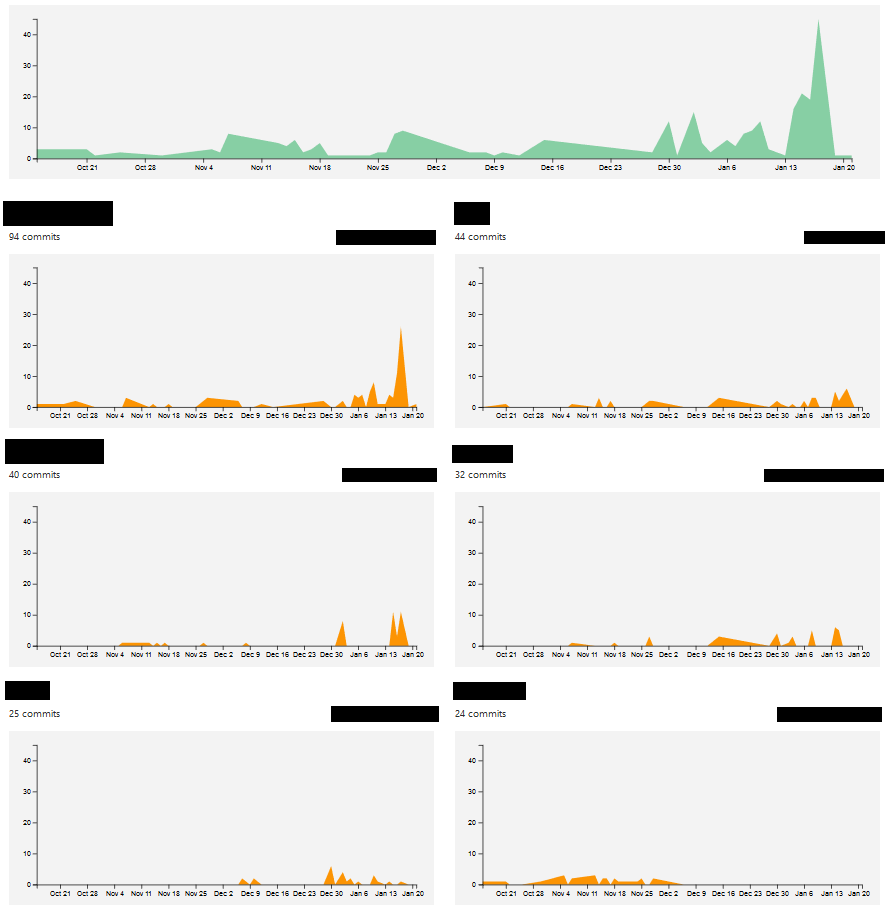
\includegraphics[scale=0.4]{slike/aktivnost.PNG} %veličina slike u odnosu na originalnu datoteku i pozicija slike
			\centering
			\caption{Primjer slike s potpisom}
			\label{fig:promjene}
		\end{figure}
		
		\begin{figure}[H]
			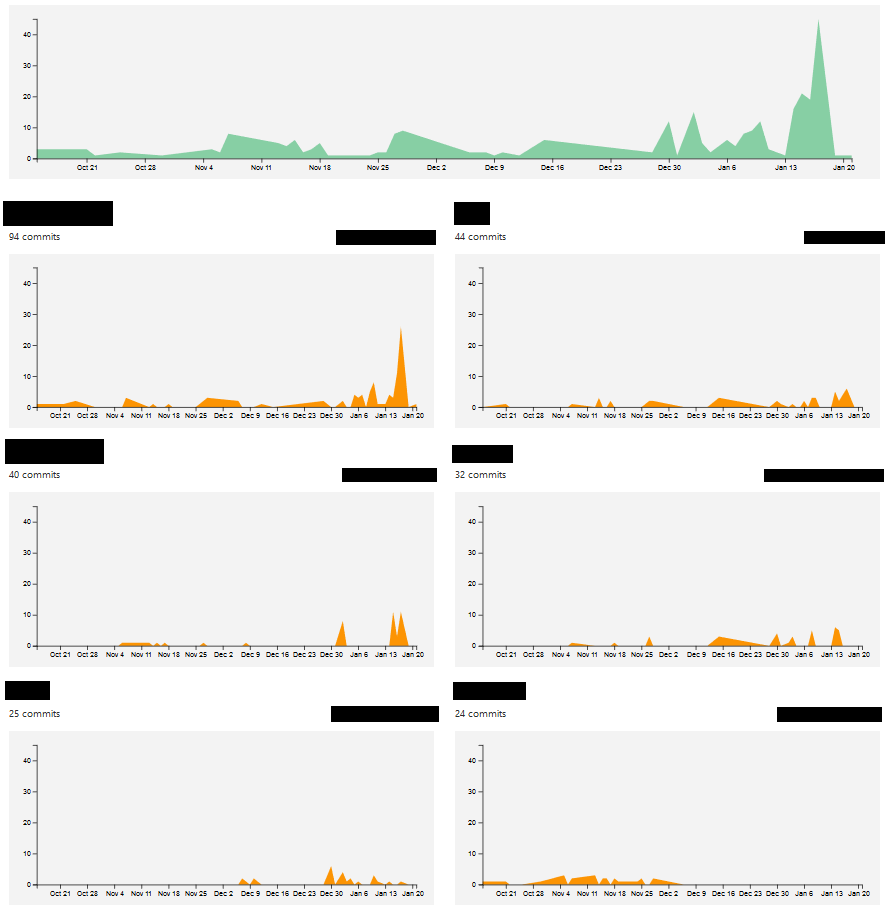
\includegraphics[width=\textwidth]{slike/aktivnost.PNG} %veličina u odnosu na širinu linije
			\caption{Primjer slike s potpisom 2}
			\label{fig:promjene2} %label mora biti drugaciji za svaku sliku
		\end{figure}
		
		Referenciranje slike \ref{fig:promjene2} u tekstu.
		
		\eject
		
	
	\chapter{Specifikacija programske potpore}
		
	\section{Funkcionalni zahtjevi}
			
			\textbf{\textit{dio 1. revizije}}\\
			
			\textit{Navesti \textbf{dionike} koji imaju \textbf{interes u ovom sustavu} ili  \textbf{su nositelji odgovornosti}. To su prije svega korisnici, ali i administratori sustava, naručitelji, razvojni tim.}\\
				
			\textit{Navesti \textbf{aktore} koji izravno \textbf{koriste} ili \textbf{komuniciraju sa sustavom}. Oni mogu imati inicijatorsku ulogu, tj. započinju određene procese u sustavu ili samo sudioničku ulogu, tj. obavljaju određeni posao. Za svakog aktora navesti funkcionalne zahtjeve koji se na njega odnose.}\\
			
			
			\noindent \textbf{Dionici:}
			
			\begin{packed_enum}
				
				\item Dionik 1
				\item Dionik 2				
				\item ...
				
			\end{packed_enum}
			
			\noindent \textbf{Aktori i njihovi funkcionalni zahtjevi:}
			
			
			\begin{packed_enum}
				\item  \underbar{Aktor 1 (inicijator) može:}
				
				\begin{packed_enum}
					
					\item funkcionalnost 1
					\item funkcionalnost 2
					\begin{packed_enum}
						
						\item  podfunkcionalnost 1 
						\item  podfunkcionalnost 2
				
					\end{packed_enum}
					\item  funkcionalnost 3
					
				\end{packed_enum}
			
				\item  \underbar{Aktor 2 (sudionik) može:}
				
				\begin{packed_enum}
					
					\item funkcionalnost 1
					\item funkcionalnost 2
					
				\end{packed_enum}
			\end{packed_enum}
			
			\eject 
			
			
				
			\subsection{Obrasci uporabe}
				
				\textbf{\textit{dio 1. revizije}}
				
				\subsubsection{Opis obrazaca uporabe}
					\textit{Funkcionalne zahtjeve razraditi u obliku obrazaca uporabe. Svaki obrazac je potrebno razraditi prema donjem predlošku. Ukoliko u nekom koraku može doći do odstupanja, potrebno je to odstupanje opisati i po mogućnosti ponuditi rješenje kojim bi se tijek obrasca vratio na osnovni tijek.}\\
					

					\noindent \underbar{\textbf{UC$<$broj obrasca$>$ -$<$ime obrasca$>$}}
					\begin{packed_item}
	
						\item \textbf{Glavni sudionik: }$<$sudionik$>$
						\item  \textbf{Cilj:} $<$cilj$>$
						\item  \textbf{Sudionici:} $<$sudionici$>$
						\item  \textbf{Preduvjet:} $<$preduvjet$>$
						\item  \textbf{Opis osnovnog tijeka:}
						
						\item[] \begin{packed_enum}
	
							\item $<$opis korak jedan$>$
							\item $<$opis korak dva$>$
							\item $<$opis korak tri$>$
							\item $<$opis korak četiri$>$
							\item $<$opis korak pet$>$
						\end{packed_enum}
						
						\item  \textbf{Opis mogućih odstupanja:}
						
						\item[] \begin{packed_item}
	
							\item[2.a] $<$opis mogućeg scenarija odstupanja u koraku 2$>$
							\item[] \begin{packed_enum}
								
								\item $<$opis rješenja mogućeg scenarija korak 1$>$
								\item $<$opis rješenja mogućeg scenarija korak 2$>$
								
							\end{packed_enum}
							\item[2.b] $<$opis mogućeg scenarija odstupanja u koraku 2$>$
							\item[3.a] $<$opis mogućeg scenarija odstupanja  u koraku 3$>$
							
						\end{packed_item}
					\end{packed_item}
				
					
				\subsubsection{Dijagrami obrazaca uporabe}
					
					\textit{Prikazati odnos aktora i obrazaca uporabe odgovarajućim UML dijagramom. Nije nužno nacrtati sve na jednom dijagramu. Modelirati po razinama apstrakcije i skupovima srodnih funkcionalnosti.}
				\eject		
				
			\subsection{Sekvencijski dijagrami}
				
				\textbf{\textit{dio 1. revizije}}\\
				
				\textit{Nacrtati sekvencijske dijagrame koji modeliraju najvažnije dijelove sustava (max. 4 dijagrama). Ukoliko postoji nedoumica oko odabira, razjasniti s asistentom. Uz svaki dijagram napisati detaljni opis dijagrama.}
				\eject
	
		\section{Ostali zahtjevi}
		
			\textbf{\textit{dio 1. revizije}}\\
		 
			 \textit{Nefunkcionalni zahtjevi i zahtjevi domene primjene dopunjuju funkcionalne zahtjeve. Oni opisuju \textbf{kako se sustav treba ponašati} i koja \textbf{ograničenja} treba poštivati (performanse, korisničko iskustvo, pouzdanost, standardi kvalitete, sigurnost...). Primjeri takvih zahtjeva u Vašem projektu mogu biti: podržani jezici korisničkog sučelja, vrijeme odziva, najveći mogući podržani broj korisnika, podržane web/mobilne platforme, razina zaštite (protokoli komunikacije, kriptiranje...)... Svaki takav zahtjev potrebno je navesti u jednoj ili dvije rečenice.}
			 
			 
			 
	
	\chapter{Arhitektura i dizajn sustava}
		
		Arhitektura se može podijeliti na tri glavna dijela:
		
		\begin{itemize}
			\item 	\textit{REST API poslužitelj (Spring Boot)}
			\item 	\textit{Klijentska aplikacija (React)}
			\item 	\textit{Baza podataka}		
		\end{itemize}
		
		\begin{figure}[h]
			\centering
			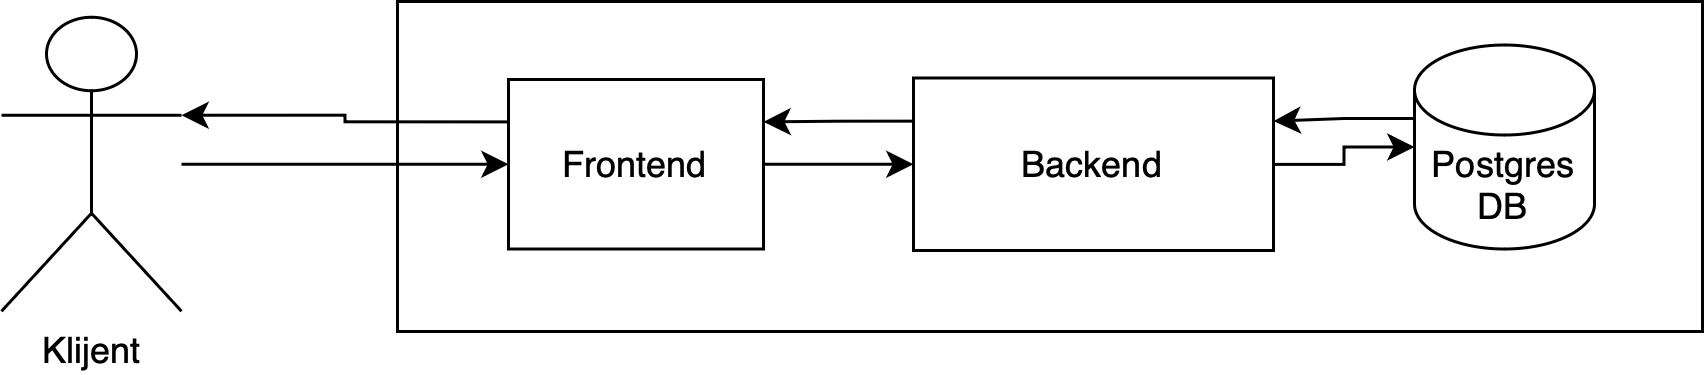
\includegraphics[width=0.8\linewidth]{./slike/arhitektura_sustava.png} 
			\caption{Arhitektura sustava}
			\label{fig:arh_sustava}
		\end{figure}
		
		
		
		Korisnik interagira s klijentskom aplikacijom putem web preglednika. Ova aplikacija je odvojena od backend sustava te koristi React uz typescript za stvaranje dinamičkog korisničkog sučelja.
		
		REST API poslužitelj izgrađen je koristeći Spring Boot, koji omogućuje izradu visoko efikasnih i skalabilnih RESTful servisa. Komunikacija između klijenta i servera odvija se putem HTTP protokola, gdje frontend šalje zahtjeve backendu, a backend odgovara s potrebnim podacima u JSON formatu.
		
		Klijentska aplikacija je odgovorna za prikazivanje podataka korisniku i obradu korisničkih interakcija. Ona komunicira s backendom putem REST API-ja za dohvaćanje i slanje podataka.
		
		Postgres baza podataka čuva sve podatke potrebne za aplikaciju. Spring Boot aplikacija komunicira s bazom podataka koristeći Spring Data JPA za upravljanje podacima.
		
		Odlučili smo se za korištenje Intellij-a kao razvojnog okruženja za backend, a za frontend koristimo Visual Studio Code.
		Za razliku od tradicionalnog MVC koncepta, naš sustav je podijeljen na odvojene slojeve gdje backend (REST API poslužitelj) i frontend (klijentska aplikacija) rade neovisno jedan o drugome. Uspoređujući s tradicionalnim MVC konceptom, mogli bismo reći da je View (V u MVC) na frontendu, a Model I Controller (M I C u MVC) na backendu. Ovo omogućuje fleksibilnost i lakše skaliranje svakog dijela aplikacije zasebno.
				

				
		\section{Baza podataka}

			Za potrebe naše aplikaicje korisiti ćemo relacijsku bazu podataka kako bismo lakše oblikovali stvarni svijet. Baza nam je potrbna za metodičku pohranu podataka te njihovo brzo dohvaćanje. Naša baza podataka se sastoji od sljedećih entiteta:
			
			\begin{packed_item}
				\item Patient
				\item Accommodation
				\item AccommodationOrder
				\item AccommodationBooking
				\item TransportCompany
				\item TransportVehicle
				\item TransportBooking
				\item MedicalAppointment
				\item AdminRole
				\item AdminRoles
				\item Admin
			\end{packed_item}
		
			\subsection{Opis tablica}
			
				
				\noindent
				\textbf{Patient} Ova entitet sadrži sve informacije o korisniku usluga našeg sustava. Kako su svi korisnici pacijenti odlučili smo ih imenovati tako. Entitet sadrži atribute: patient\_ID, first\_name, last\_name, PIN, email i phone\_number. Ovaj entitet je u vezi \textit{One-to-Many} s entitetom AccommodationOrder preko atributa patient\_ID i u \textit{One-to-Many} s entitetom AccommodationBooking preko atributa patient\_ID.
				
				\begin{longtblr}[
					label=none,
					entry=none
					]{
						width = \textwidth,
						colspec={|X[6,l]|X[6, l]|X[20, l]|}, 
						rowhead = 1,
					} %definicija širine tablice, širine stupaca, poravnanje i broja redaka naslova tablice
				
					\hline 
					\SetCell[c=3]{c}{\textbf{Patient}}\\
					\hline[3pt]
					\SetCell{LightGreen}patient\_ID & VARCHAR & primarni ključ tablice \\
					\hline
					first\_name	& VARCHAR &  ime pacijenta\\ 
					\hline 
					last\_name & VARCHAR &  prezime pacijenta \\ 
					\hline 
					PIN & VARCHAR	&  Personal Identification Number, kao OIB u hrvatskoj\\ 
					\hline 
					email & VARCHAR & pacijentov email\\ 
					\hline	
					phone\_number & VARCHAR & pacijentov telefonski broj \\
					\hline
				\end{longtblr}
			
				\noindent
				\textbf{Accommodation} Ovaj entitet sadržava potrebne podatke o nekom smještaju koji je smještajni administrator unio. Entitet sadrži atribute: accommodation\_ID, type, category, address, availibility\_start, availability\_end i location. Ovaj entitet je u \textit{One-to-Many} vezi s entitetom AccommodationBooking preko atributa accommodation\_ID.
				
				\begin{longtblr}[
					label=none,
					entry=none
					]{
						width = \textwidth,
						colspec={|X[10,l]|X[6, l]|X[18, l]|}, 
						rowhead = 1,
					} %definicija širine tablice, širine stupaca, poravnanje i broja redaka naslova tablice
					\hline 
					\SetCell[c=3]{c}{\textbf{Accommodation}}\\ 
					\hline[3pt]
					\SetCell{LightGreen}accommodation\_ID & VARCHAR & primarni ključ tablice\\ 
					\hline
					type & VARCHAR & versta smještaja \\
					\hline 
					category & VARCHAR & kategorija smještaja \\
					\hline
					address & VARCHAR & adresa smještaja \\
					\hline
					availability\_start & DATETIME & datum i vrijeme od kada je smještaj dostupan \\
					\hline
					availability\_end & DATETIME & datum i vrijeme do kada je smještaj dosupan \\
					\hline
					location & POINT & kordinate smještaja \\
					\hline
				\end{longtblr}
			
			\noindent
			\textbf{AccommodationOrder} Ovaj entitet se koristi za pohravnjivanje pacijentovih zahtjeva o traženom smještaju. U slučaju da traženi smještaj nije odmah dostupan zahtjev se sprema kako bih se kasnije mogao opet pogledati. Entitet sadrži atribute: accommodation\_order\_ID, arrival\_datetime, departure\_datetime, accommodation\_type, accommodation\_category i patient\_ID. Ovaj entitet je u \textit{Many-to-One} vezi s entitetom Patient preko patient\_ID atributa.
			\begin{longtblr}[
				label=none,
				entry=none
				]{
					width = \textwidth,
					colspec={|X[13,l]|X[6, l]|X[20, l]|}, 
					rowhead = 1,
				} %definicija širine tablice, širine stupaca, poravnanje i broja redaka naslova tablice
				\hline 
				\SetCell[c=3]{c}{\textbf{AccommodationOrder}}\\ 
				\hline[3pt]
				\SetCell{LightGreen}accommodation\_order\_ID & VARCHAR & primarni ključ tablice\\ 
				\hline
				arrival\_datetime & DATETIME & vrijeme dolaska pacijenta u državu, od tada mu treba smještaj\\
				\hline
				departure\_datetime & DATETIME & vrijeme odlaska pacijenta iz države, do tada treba smještaj \\
				\hline
				accommodation\_type & VARCHAR & željeni tip smještaja koji pacijent traži \\
				\hline
				accommodation\_category & VARCHAR & željena kategorija smještaja koju pacijent traži \\
				\hline
				\SetCell{LightBlue} patient\_ID	& STRING & ID pacijenta koji je napravio ovaj zahtjev \\
				\hline 
			\end{longtblr}
			
			\noindent
			\textbf{AccommodationBooking} Ovaj vezni entitet se koristi za pohranjivanje informacije koji pacijent je kada u kojem smještaju. Entitet sadrži atribute: accommodation\_booking\_ID, start\_datetime, end\_datetime, accommodation\_ID, patient\_ID. Ovaj entitet je u \textit{Many-to-One} vezi s entitetom Accommodation preko atributa accommodation\_ID. U \textit{Many-to-One} vezi s entitetom Patient preko atributa patient\_ID. I u \textit{One-to-Many} s entitetom TransportBooking preko accommodation\_booking\_ID.
			\begin{longtblr}[
				label=none,
				entry=none
				]{
					width = \textwidth,
					colspec={|X[10, l]|X[6, l]|X[20, l]|}, 
					rowhead = 1,
				} %definicija širine tablice, širine stupaca, poravnanje i broja redaka naslova tablice
				\hline 
				\SetCell[c=3]{c}{\textbf{AccommodationBooking}}\\ 
				\hline[3pt]
				\SetCell{LightGreen}accommodation\_
				booking\_ID & VARCHAR & primarni ključ tablice \\ 
				\hline
				start\_datetime & DATETIME & datum i vrijeme od kada je pacijent u smještaju \\
				\hline
				end\_datetime & DATETIME & datum i vrijeme do kada je pacijent u smještaju \\
				\hline 
				\SetCell{LightBlue} accommodation\_ID	& VARCHAR & smještaj u koji je pacijent smješten \\
				\hline 
				\SetCell{LightBlue} patient\_ID & VARCHAR & pacijent koji ostaje u smještaju \\
				\hline
			\end{longtblr}
			
			\noindent
			\textbf{TransportCompany} Ovaj entitet sadržava informacije o transportnoj firmi. Entitet sadrži atribute: transport\_company\_ID, name, phone\_number, email. Ovaj entitet je u \textit{One-to-Many} vezi s entitetom TransportVehicle preko atributa transport\_company\_ID.
			\begin{longtblr}[
				label=none,
				entry=none
				]{
					width = \textwidth,
					colspec={|X[11,l]|X[6, l]|X[20, l]|}, 
					rowhead = 1,
				} %definicija širine tablice, širine stupaca, poravnanje i broja redaka naslova tablice
				\hline 
				\SetCell[c=3]{c}{\textbf{TransportCompany}}\\ 
				\hline[3pt]
				\SetCell{LightGreen}transport\_company\_ID & VARCHAR & primarni ključ tablice \\ 
				\hline
				name & VARCHAR & ime firme \\
				\hline 
				phone\_number & VARCHAR & felefonski broj firme \\
				\hline
				email & VARCHAR & email firme \\
				\hline 
			\end{longtblr}
			
			\noindent
			\textbf{TransportVehicle} Ovaj entitet sadržava informacije o nekom transportnom vozilu. Entitet sadrži atribute: transport\_comapny\_ID, name, phone\_number, email. Ovaj entitet je u \textit{Many-to-One} vezi s entitetom TransportCompany preko atributa transport\_company\_ID. I u \textit{One-to-Many} vezi s entitetom TransportBooking preko atributa transport\_vehicle\_ID.
			\begin{longtblr}[
				label=none,
				entry=none
				]{
					width = \textwidth,
					colspec={|X[11,l]|X[6, l]|X[20, l]|}, 
					rowhead = 1,
				} %definicija širine tablice, širine stupaca, poravnanje i broja redaka naslova tablice
				\hline 
				\SetCell[c=3]{c}{\textbf{TransportVehicle}}\\ 
				\hline[3pt]
				\SetCell{LightGreen}transport\_vehicle\_ID & VARCHAR & primarni ključ tablice \\ 
				\hline
				type & VARCHAR & vrsta vozila \\
				\hline 
				capacity & INT & kapacitet vozila \\
				\hline
				\SetCell{LightBlue} transport\_company\_ID	& VARCHAR & transportna firma kojoj pripada ovo vozilo \\
				\hline 
			\end{longtblr}
			
			\noindent
			\textbf{TransportBooking} Ovo je slabi vezni entitet koji označava prijevoz pacijenta. Ujedinjuje tri entiteta iz kojih saznajem kojeg pacijenta treba voziti, od kuda će biti transportiran, koje vozilo će se korisiti i do koje klinike će se transportirati. Entitet sadrži atribute: transport\_vehicle\_ID, accommodation\_booking\_ID, medical\_appointment\_ID. Entitet je u \textit{Many-to-One} vezi s entitetom TransportVehicle preko atributa transport\_vehicle\_ID. U \textit{Many-to-One} vezi s entitetom AccommodationBooking preko atributa accommodaton\_booking\_ID. I u \textit{Many-to-One} vezi s entitetom MedicalAppointment preko atributa medical\_appointment\_ID.
			\begin{longtblr}[
				label=none,
				entry=none
				]{
					width = \textwidth,
					colspec={|X[11,l]|X[6, l]|X[20, l]|}, 
					rowhead = 1,
				} %definicija širine tablice, širine stupaca, poravnanje i broja redaka naslova tablice
				\hline 
				\SetCell[c=3]{c}{\textbf{TransportBooking}}\\ 
				\hline[3pt]
				\SetCell{LightBlue} transport\_vehicle\_ID & VARCHAR & vozilo koje obavlja ovaj projevoz \\
				\hline 
				\SetCell{LightBlue} accommodation\_
				booking\_ID & VARCHAR & poveznica na smještaj i pacijenta koje treba prevesti iz tog smještaja \\
				\hline
				\SetCell{LightBlue} medical\_
				appointment\_ID & VARCHAR & poveznica na medicinski tretman koji nam daje informaciju gdje pacijenta treba voziti \\
				\hline
			\end{longtblr}
			
			\noindent
			\textbf{MedicalAppointment} Ovaj entitet korisimo za spremanje podataka o medicinskim tretmanima nekog pacijenta. Informacije o ovom ćemo dobiti iz medicinskog sustava, ali ako nije moguće odmah napravit TransportBooking zbog npr. nedostatka vozila, želimo pospremiti informacije o tretmanu. Entitet sadrži atribute: medical\_appointment\_ID, PIN, clinic\_address, start\_datetime, end\_datetime. Entitet je u \textit{One-to-One} vezi s entitetom TransportBooking preko atributa medical\_appointment\_ID. 
			\begin{longtblr}[
				label=none,
				entry=none
				]{
					width = \textwidth,
					colspec={|X[10,l]|X[6, l]|X[20, l]|}, 
					rowhead = 1,
				} %definicija širine tablice, širine stupaca, poravnanje i broja redaka naslova tablice
				\hline 
				\SetCell[c=3]{c}{\textbf{MedicalAppointment}}\\ 
				\hline[3pt]
				\SetCell{LightGreen}medical\_
				appointment\_ID & VARCHAR & primarni ključ tablice \\ 
				\hline
				PIN & VARCHAR & Personal Identification Number pacijenta za kojeg je ovo medicinski tretman \\
				\hline 
				clinic\_address & VARCHAR & adresa klinike u kojoj je tretman \\
				\hline
				start\_datetime & DATETIME & datum i vrijeme početka tretmana \\
				\hline
				end\_datetime & DATETIME & datum i vrijeme kraja tretmana \\
				\hline
			\end{longtblr}
			
			\noindent
			\textbf{AdminRole} Ovaj entitet označava role admina. Sadrži atribute, admin\_role\_ID i name. Entitet je u \textit{One-to-Many} vezi s entitetom AdminRoles preko atributa admin\_role\_ID. 
			\begin{longtblr}[
				label=none,
				entry=none
				]{
					width = \textwidth,
					colspec={|X[6,l]|X[6, l]|X[20, l]|}, 
					rowhead = 1,
				} %definicija širine tablice, širine stupaca, poravnanje i broja redaka naslova tablice
				\hline 
				\SetCell[c=3]{c}{\textbf{AdminRole}}\\ 
				\hline[3pt]
				\SetCell{LightGreen}admin\_role\_ID & VARCHAR & primarni ključ tablice \\ 
				\hline
				name & VARCHAR & deskriptivni naziv role \\
				\hline 
			\end{longtblr}
		
			
			\noindent
			\textbf{Admin} Ovaj entitet sadrži podatke o adminima. Entitet sadrži atribute: admin\_ID, email, first\_name, last\_name. Entitet je u \textit{One-to-Many} vezi s entitetom AdminRoles preko atributa admin\_ID. 
			\begin{longtblr}[
				label=none,
				entry=none
				]{
					width = \textwidth,
					colspec={|X[6,l]|X[6, l]|X[20, l]|}, 
					rowhead = 1,
				} %definicija širine tablice, širine stupaca, poravnanje i broja redaka naslova tablice
				\hline 
				\SetCell[c=3]{c}{\textbf{Admin}}\\ 
				\hline[3pt]
				\SetCell{LightGreen}admin\_ID & VARCHAR & primarni ključ tablice \\ 
				\hline
				email & VARCHAR & email admina \\
				\hline 
				first\_name & VARCHAR & ime admina \\
				\hline
				last\_name & VARCHAR & prezime admina \\
				\hline 
			\end{longtblr}
			
			\noindent 
			\textbf{AdminRoles} Ovaj vezni entitet služi kao spoj nekog admina s njegovom rolom. Atributi entiteta su: admin\_role\_ID i admin\_ID. Entitet je u \textit{Many-to-One} vezi s entitetom AdminRole preko atributa admin\_role\_ID. I entitet je u \textit{Many-to-One} vezi s entitetom Admin preko atributa admin\_ID.
			\begin{longtblr}[
				label=none,
				entry=none
				]{
					width = \textwidth,
					colspec={|X[6,l]|X[6, l]|X[20, l]|}, 
					rowhead = 1,
				} %definicija širine tablice, širine stupaca, poravnanje i broja redaka naslova tablice
				\hline 
				\SetCell[c=3]{c}{\textbf{AdminRoles}}\\ 
				\hline[3pt]
				\SetCell{LightBlue}admin\_role\_ID	& VARCHAR & poveznica na rolu ovog admina \\
				\hline 
				\SetCell{LightBlue}admin\_ID & VARCHAR & poveznica na kojeg admina se odnosi ova rola \\
				\hline
			\end{longtblr}			
				
			
			\subsection{Dijagram baze podataka}

				\begin{figure}[H]
					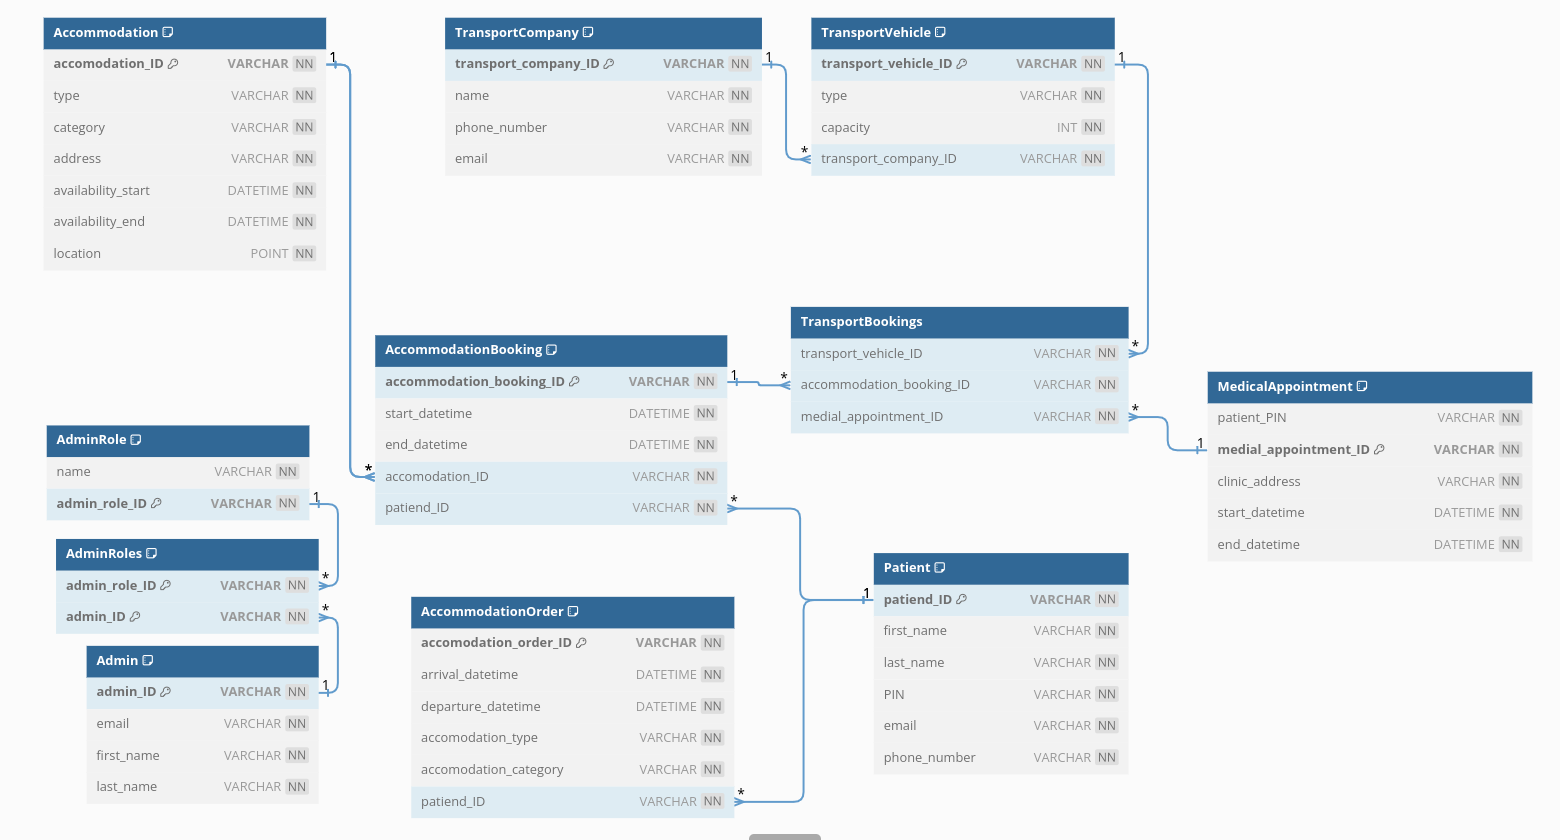
\includegraphics[scale=0.32]{slike/dijagram_baze.png} %veličina slike u odnosu na originalnu datoteku i pozicija slike
					\centering
					\caption{ER Dijagram baze podataka}
					\label{fig:dijagram_baze_podataka}
				\end{figure}
			
			\eject
			
			
		\section{Dijagram razreda}
		
			Na slikama \ref{fig:arhitektura_controller_class_diagram}  do \ref{fig:arhitektura_model_class_diagram}  prikazani su ključni elementi backend dijela arhitekture DentAll aplikacije. 
			
			Prva slika \ref{fig:arhitektura_controller_class_diagram}  prikazuje dijagram razreda svih Controller razreda koji se koriste u našoj aplikaciji.  Slika \ref{fig:arhitektura_dto_class_diagram} fokusira se na dijagram razreda s DTO razredima koje služe za prijenos podataka između Controllera i Modela. Svaka DTO klasa odgovara određenom razredu iz Modela, osiguravajući učinkovit prijenos podataka unutar aplikacije. Na slici \ref{fig:arhitektura_requests_class_diagram} nalaze se Requests razredi koje predstavljaju zahtjeve od klijenta prema Controller razredima. Ovi razredi sadrže sve potrebne informacije za izvođenje funkcionalnosti poput CREATE i UPDATE. Obuhvaćajući sve domain razrede iz modela DentAll aplikacije, dijagram razreda sa slike  \ref{fig:arhitektura_model_class_diagram} prikazuje relacije i međusobnu povezanost između razreda unutar modela. 
			
						
			\begin{figure}[H]
				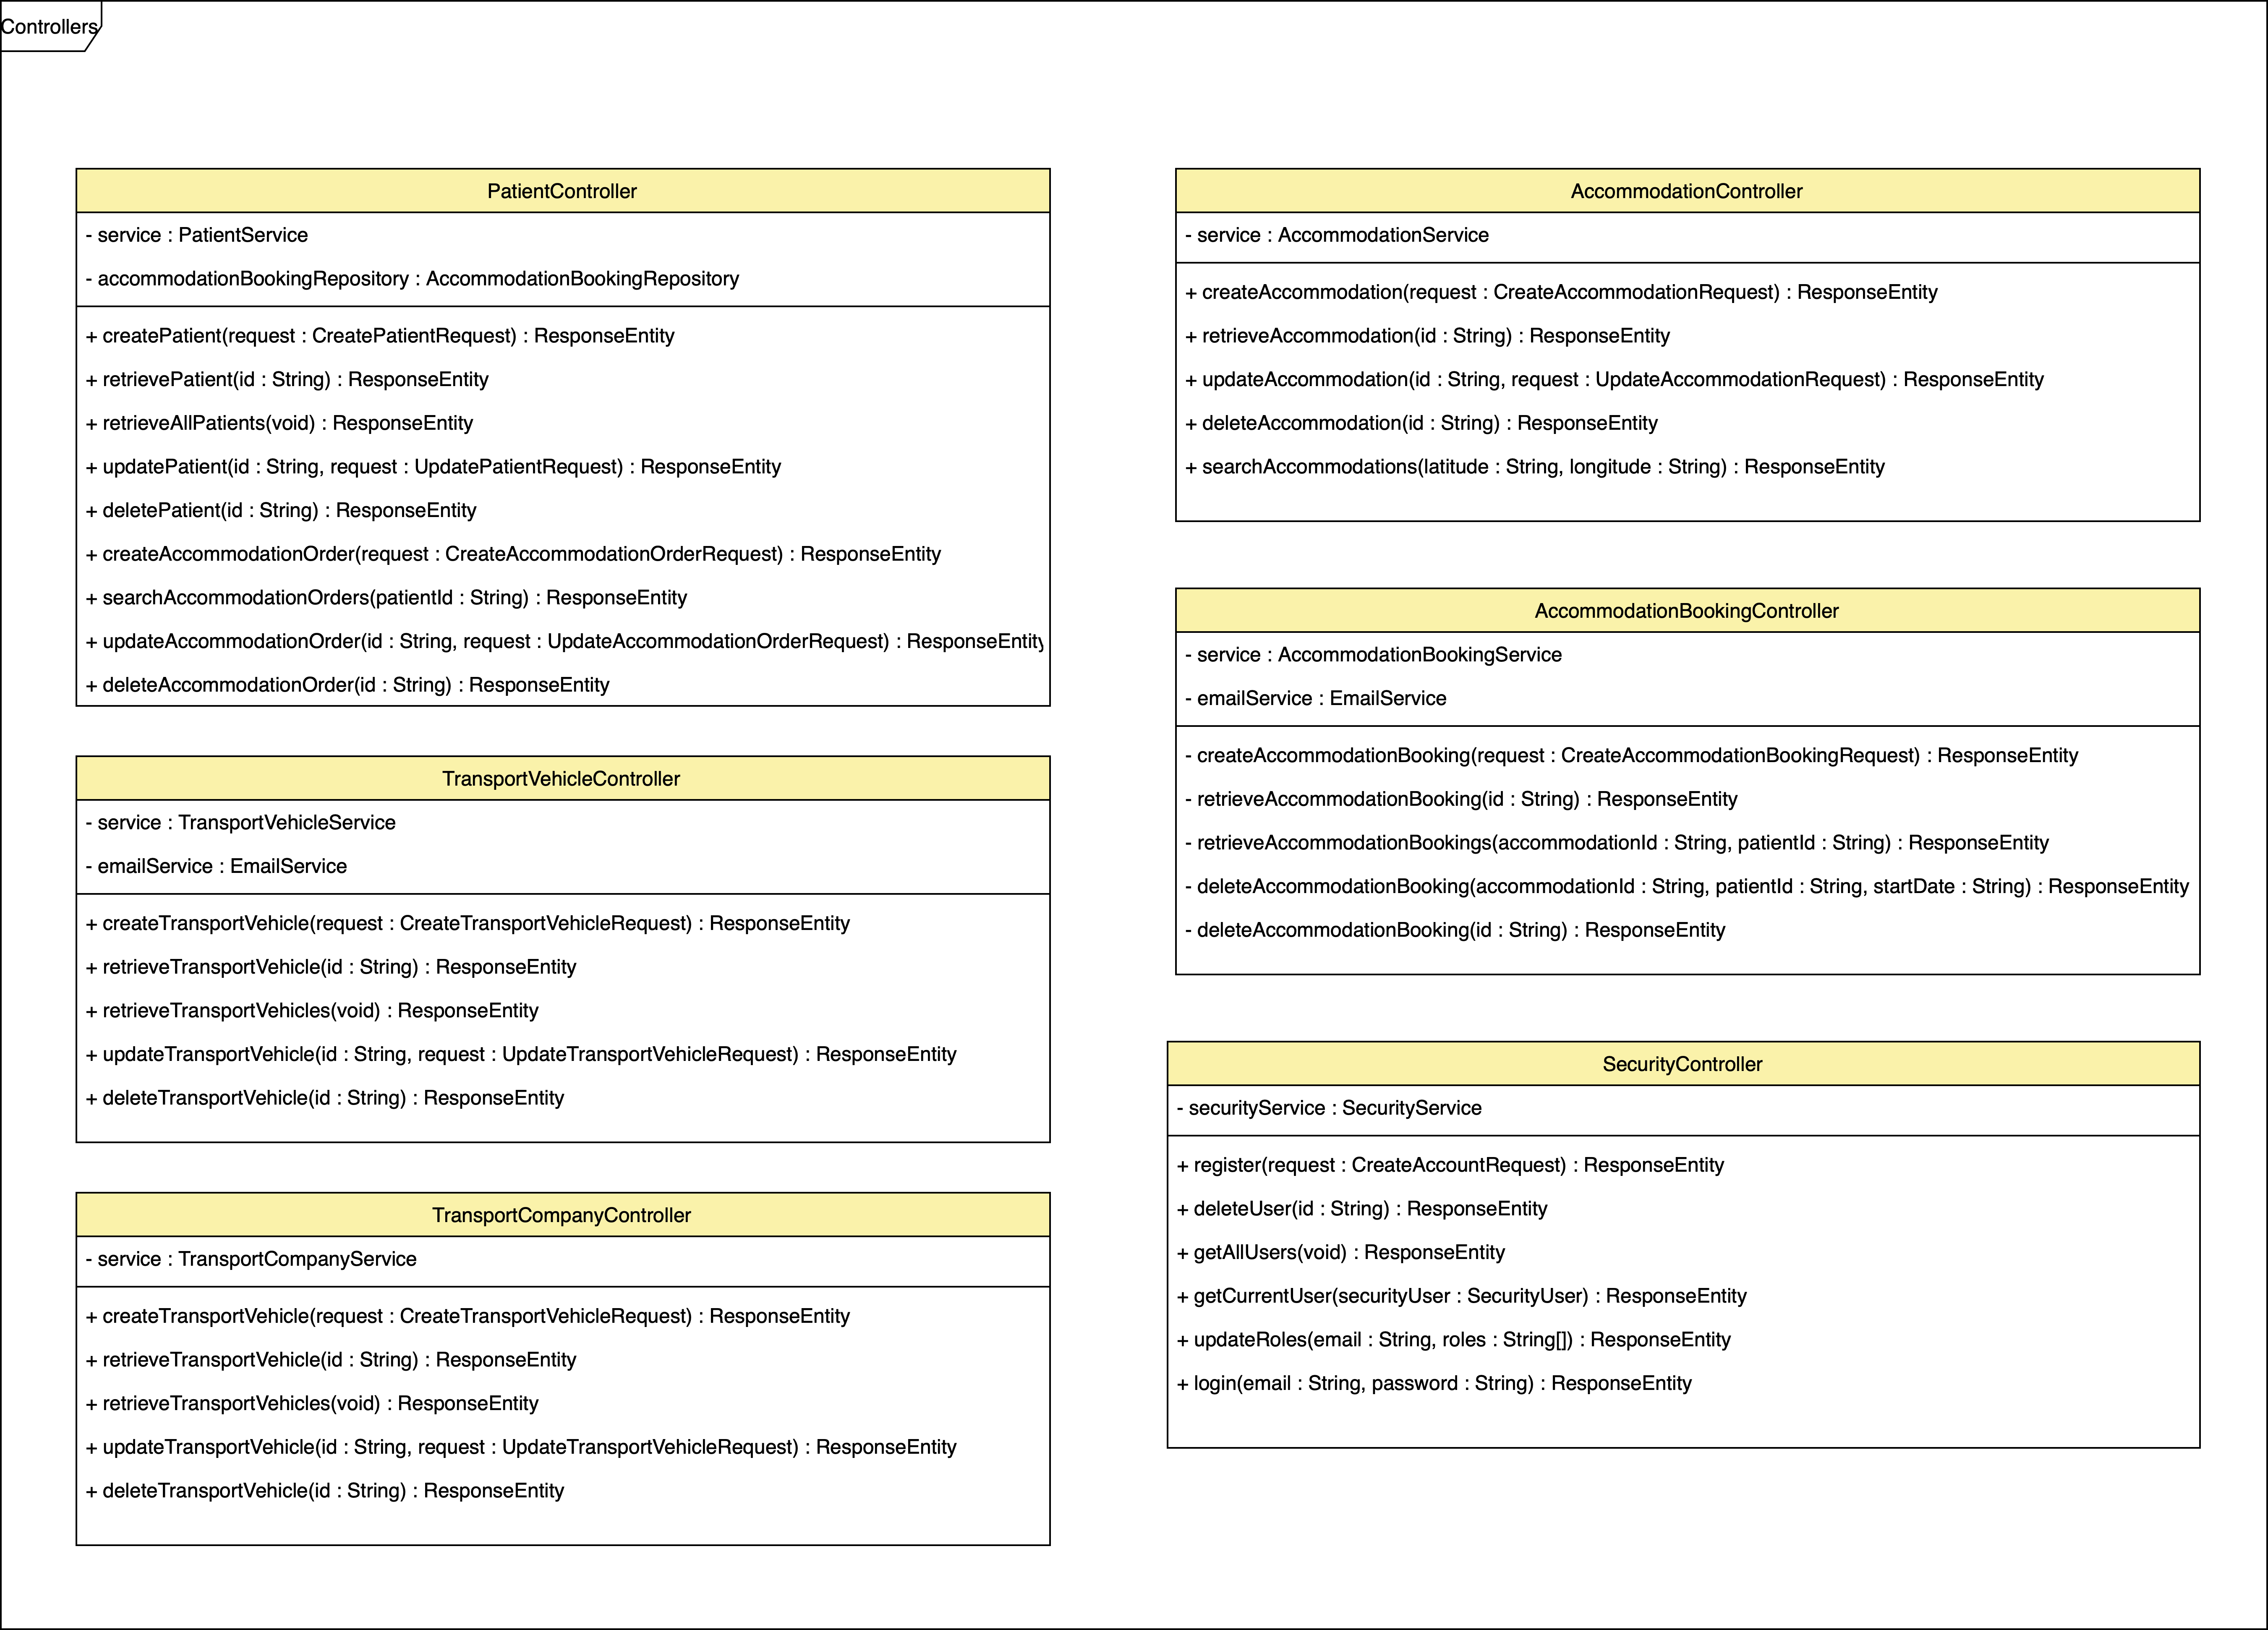
\includegraphics[scale=0.07]{slike/arhitektura_controller_class_diagram_v2.png} %veličina slike u odnosu na originalnu datoteku i pozicija slike
				\centering
				\caption{Dijagram razreda - dio Controllers}
				\label{fig:arhitektura_controller_class_diagram}
			\end{figure}
			
			\begin{figure}[H]
				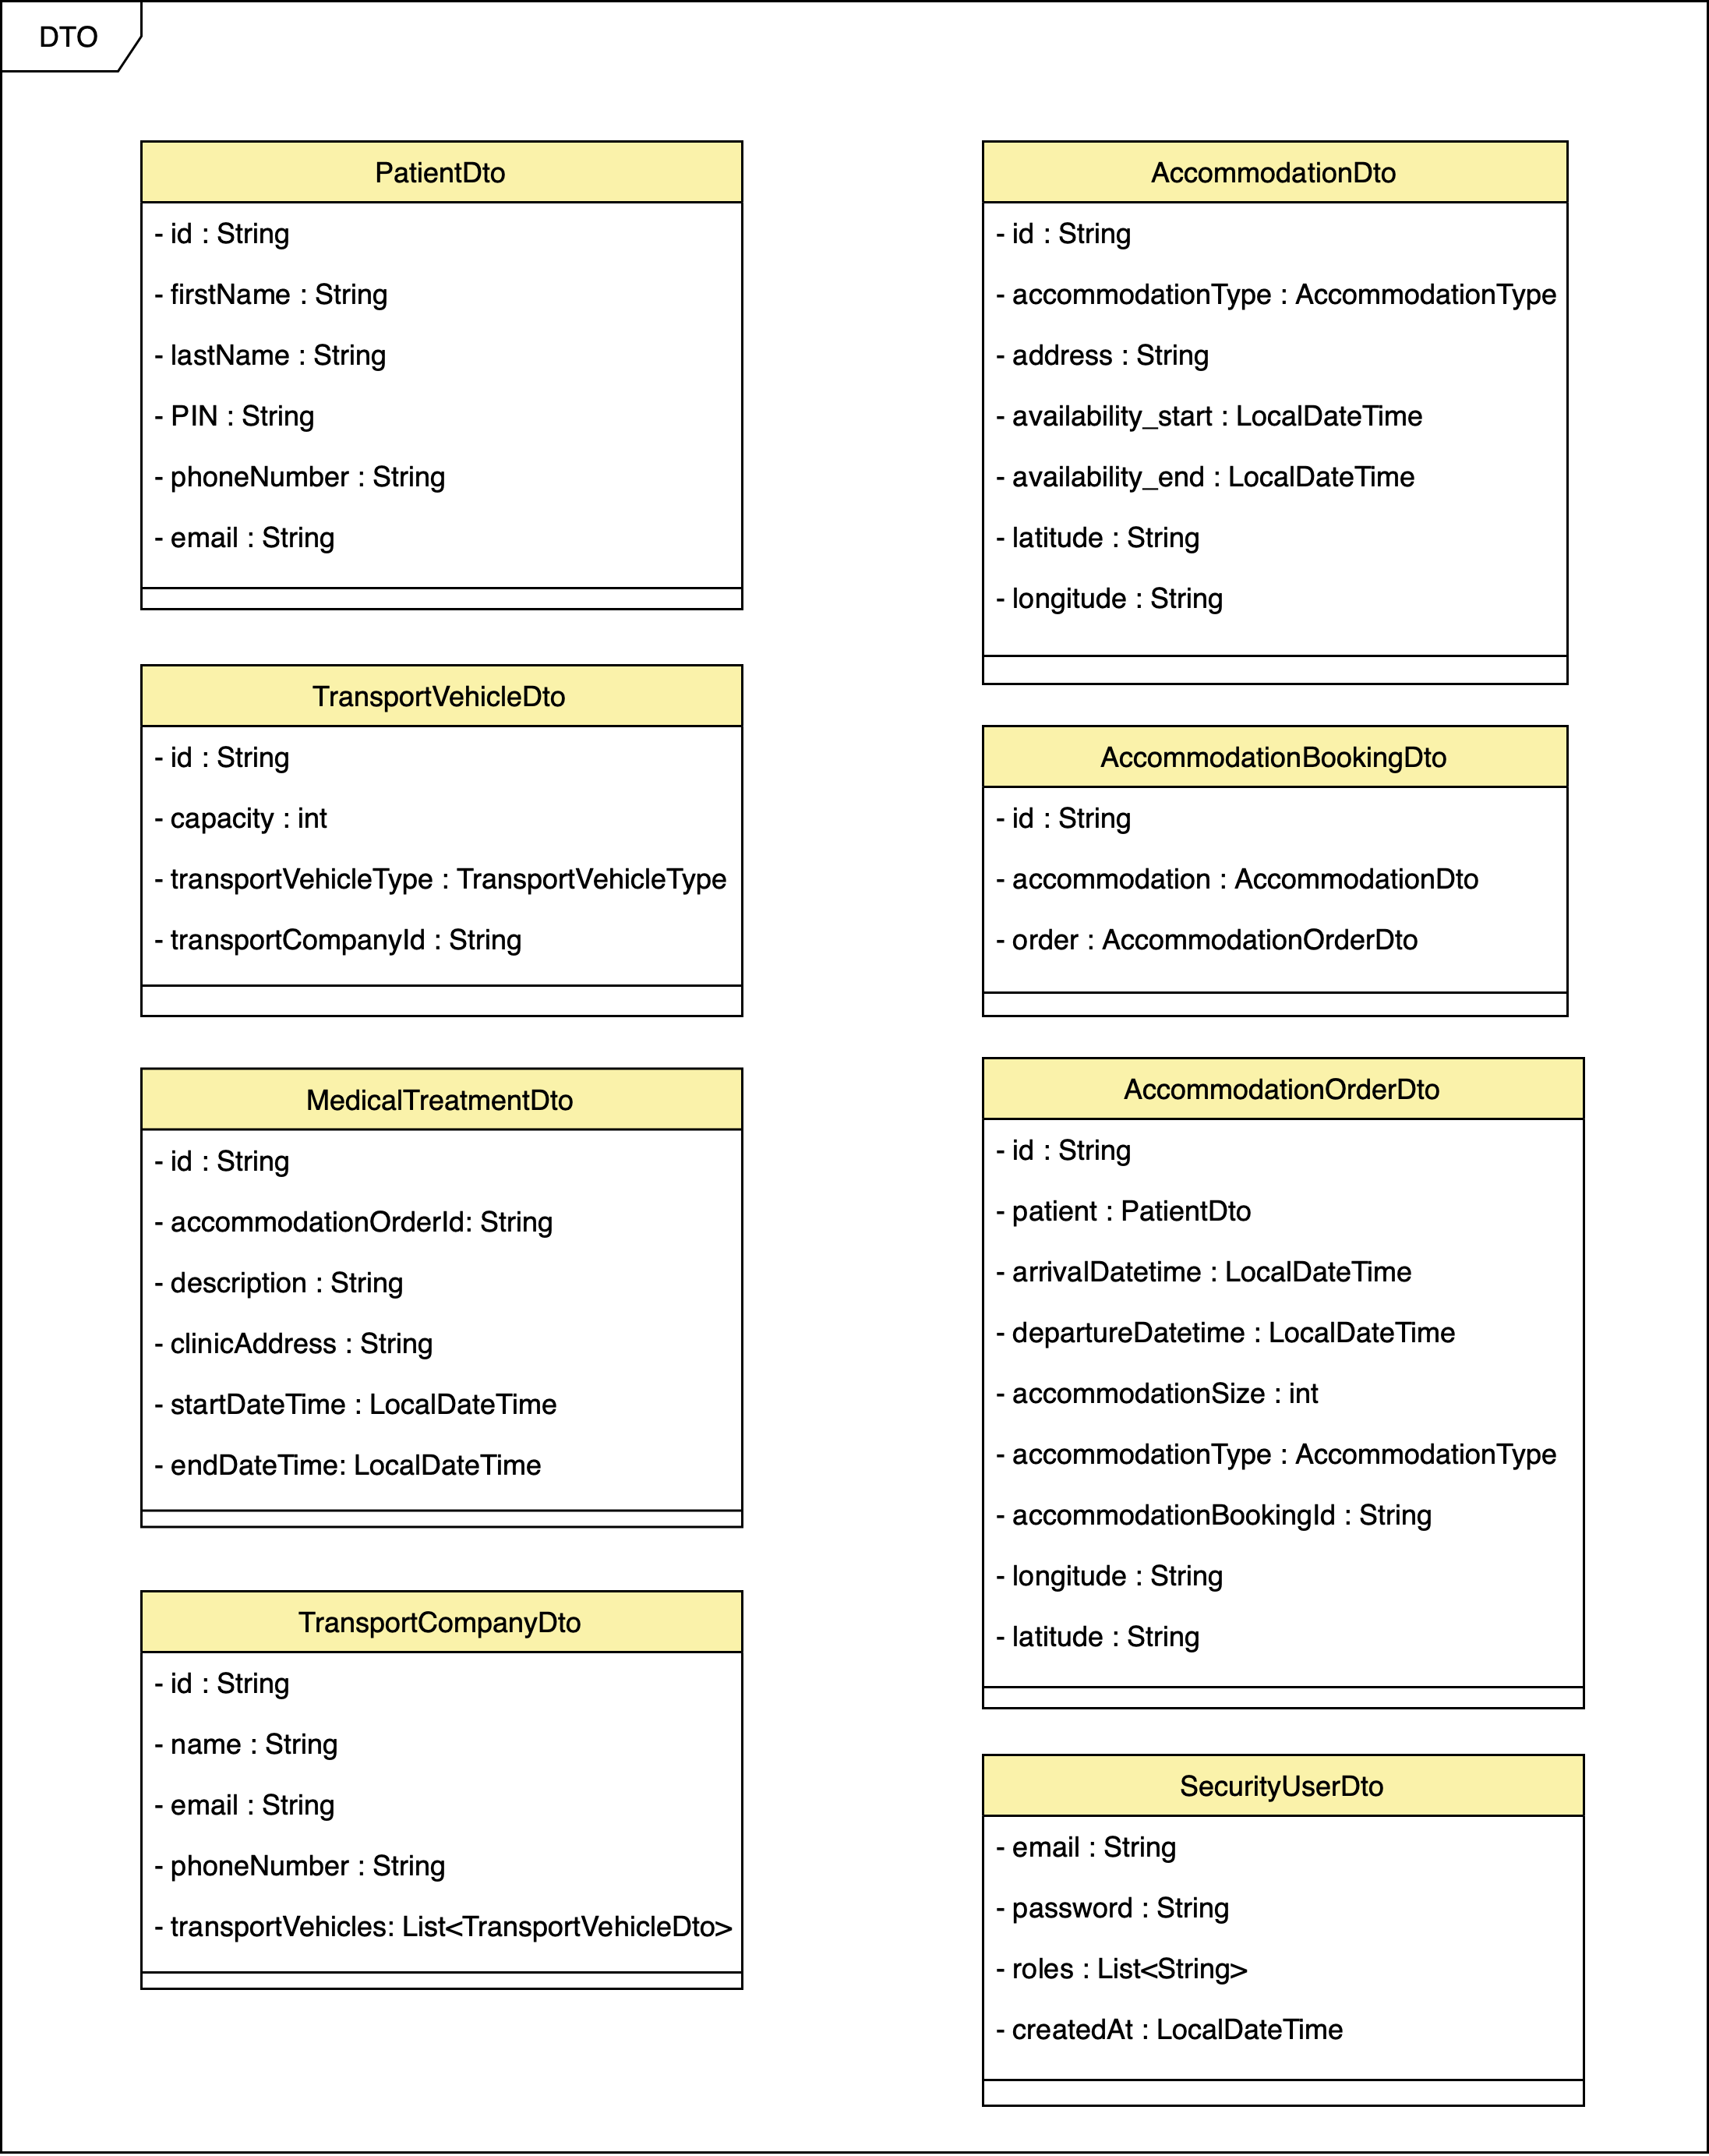
\includegraphics[scale=0.12]{slike/arhitektura_dto_class_diagram_v2.png} %veličina slike u odnosu na originalnu datoteku i pozicija slike
				\centering
				\caption{Dijagram razreda - dio DTO}
				\label{fig:arhitektura_dto_class_diagram}
			\end{figure}
			
			\begin{figure}[H]
				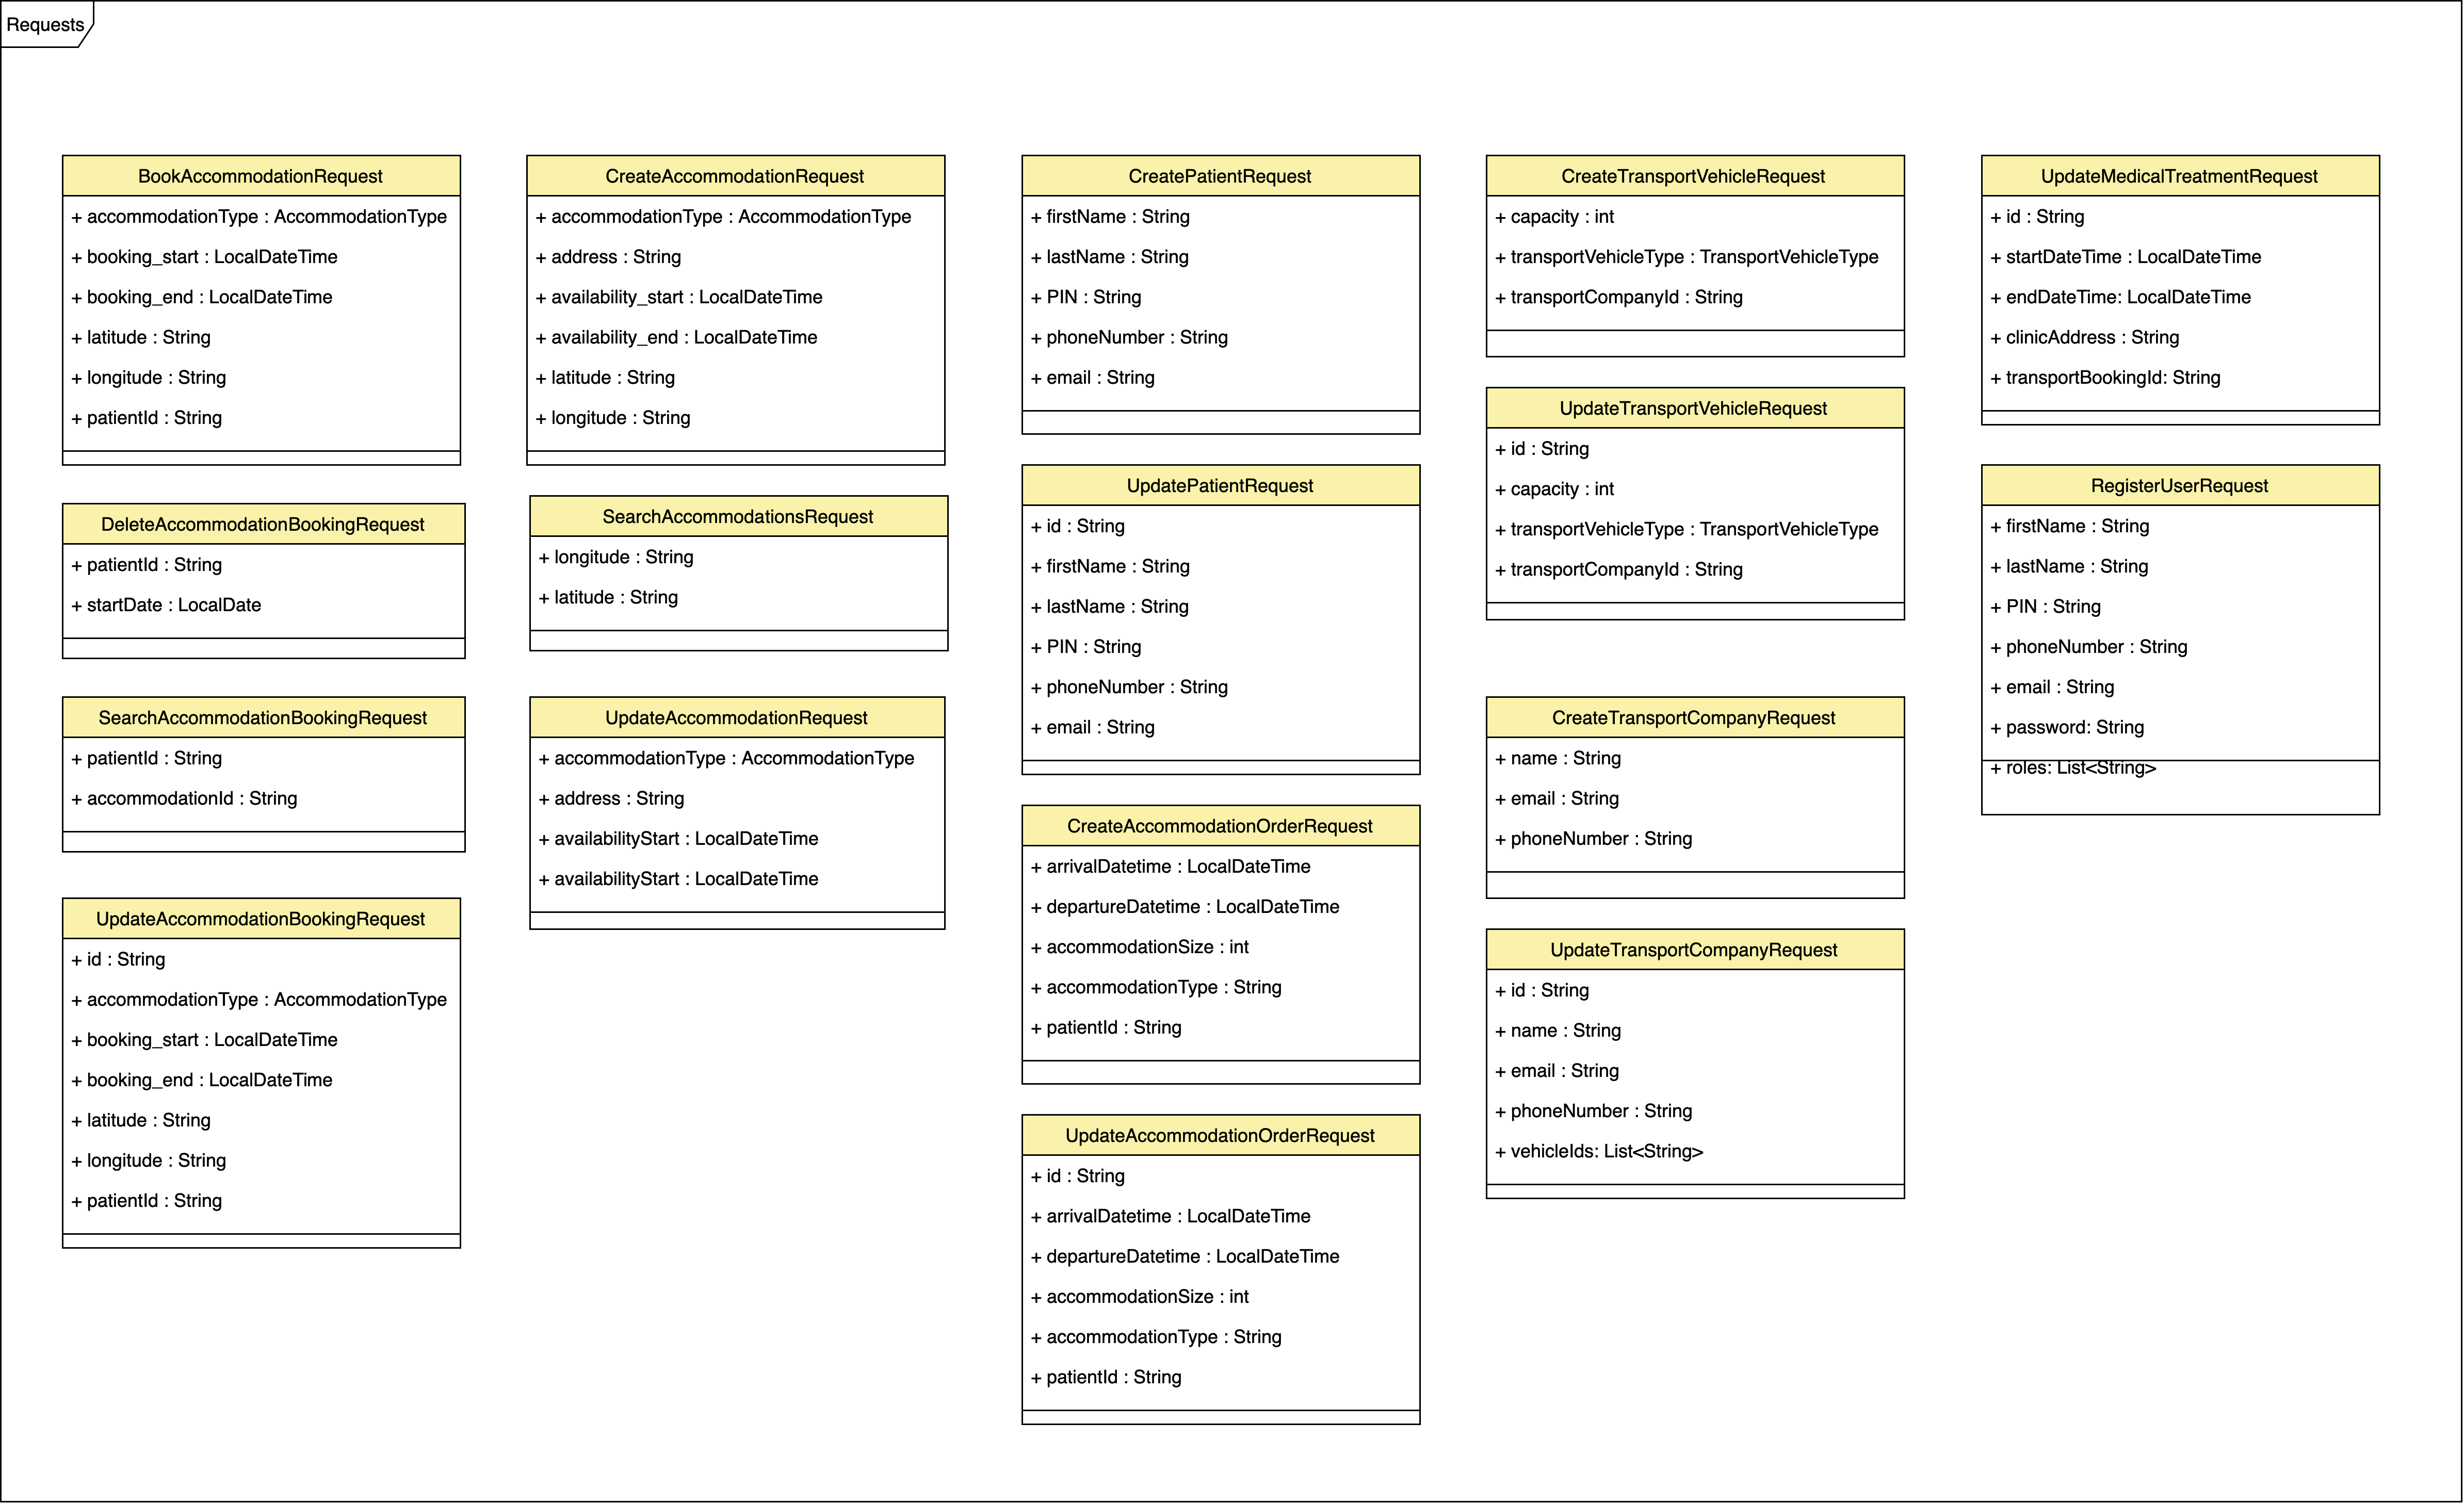
\includegraphics[scale=0.08]{slike/arhitektura_requests_class_diagram.png} %veličina slike u odnosu na originalnu datoteku i pozicija slike
				\centering
				\caption{Dijagram razreda - dio Requests}
				\label{fig:arhitektura_requests_class_diagram}
			\end{figure}
			
			\begin{figure}[H]
				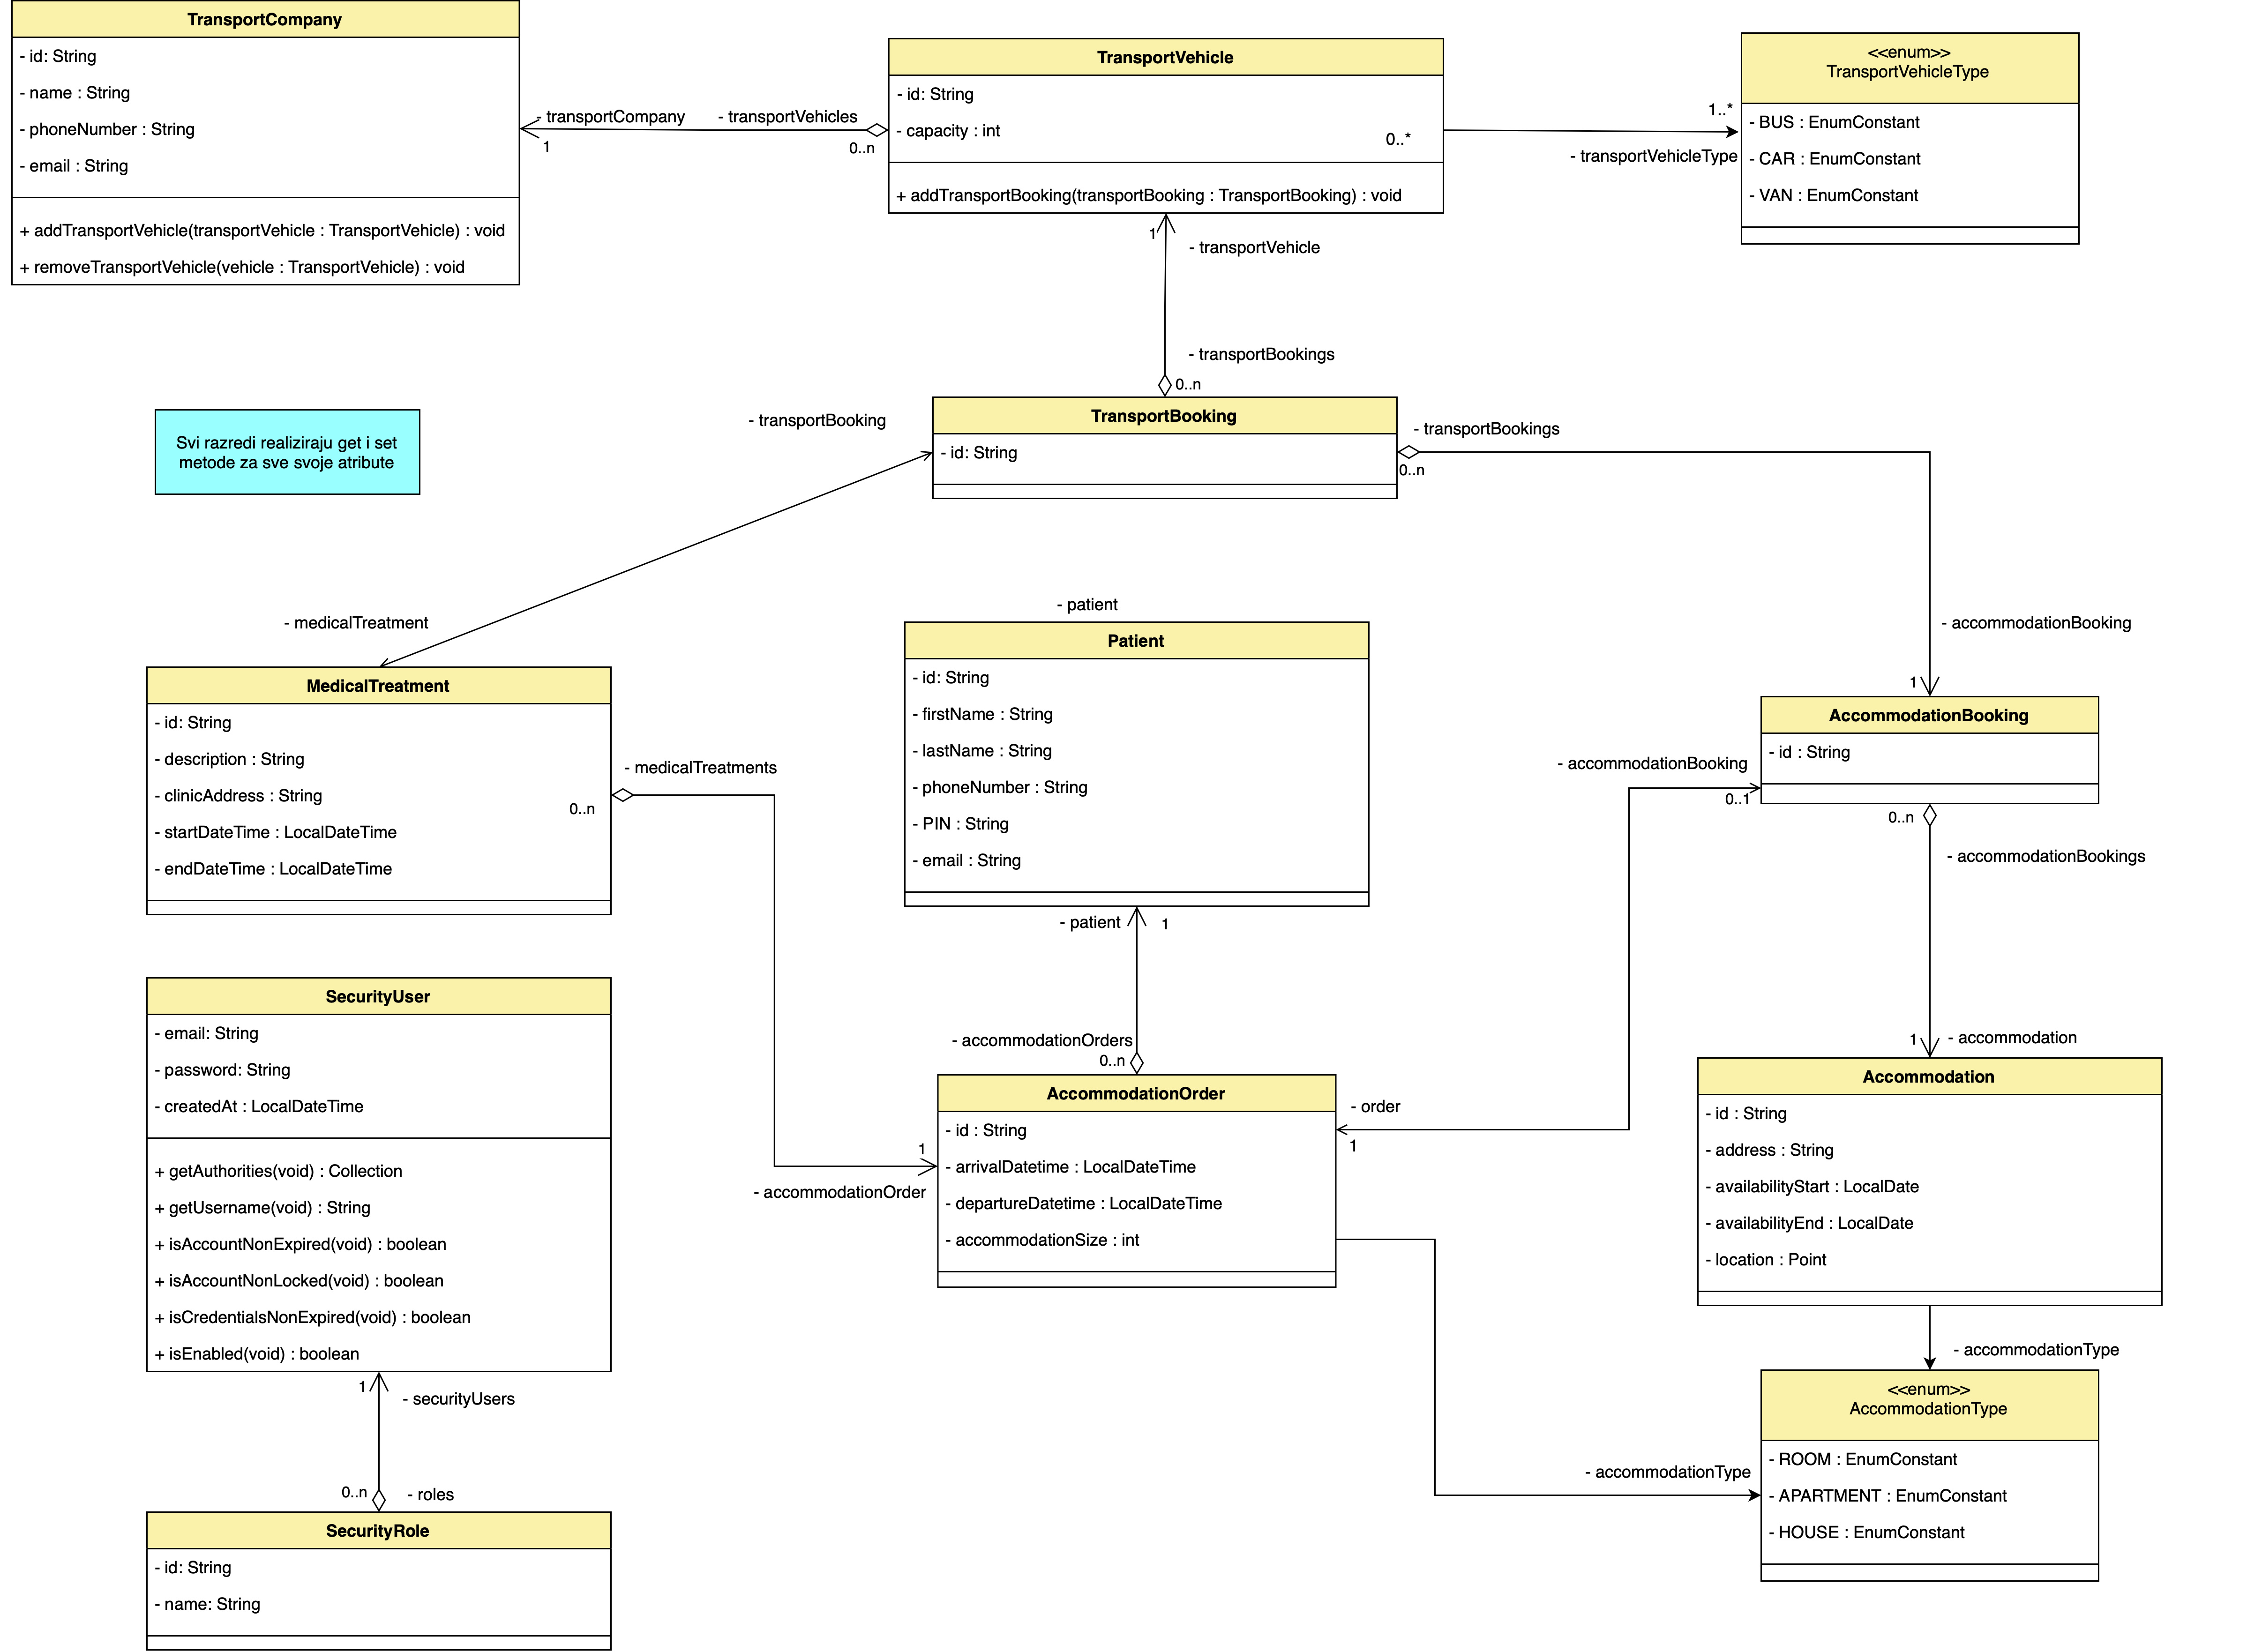
\includegraphics[scale=0.08]{slike/arhitektura_model_class_diagram_v2.png} %veličina slike u odnosu na originalnu datoteku i pozicija slike
				\centering
				\caption{Dijagram razreda - dio Model}
				\label{fig:arhitektura_model_class_diagram}
			\end{figure}
			
			
			
			\eject
		
		\section{Dijagram stanja}
			
			
			\textbf{\textit{dio 2. revizije}}\\
			
			\textit{Potrebno je priložiti dijagram stanja i opisati ga. Dovoljan je jedan dijagram stanja koji prikazuje \textbf{značajan dio funkcionalnosti} sustava. Na primjer, stanja korisničkog sučelja i tijek korištenja neke ključne funkcionalnosti jesu značajan dio sustava, a registracija i prijava nisu. }
			
			
			\eject 
		
		\section{Dijagram aktivnosti}
			
			\textbf{\textit{dio 2. revizije}}\\
			
			 \textit{Potrebno je priložiti dijagram aktivnosti s pripadajućim opisom. Dijagram aktivnosti treba prikazivati značajan dio sustava.}
			
			\eject
		\section{Dijagram komponenti}
		
			\textbf{\textit{dio 2. revizije}}\\
		
			 \textit{Potrebno je priložiti dijagram komponenti s pripadajućim opisom. Dijagram komponenti treba prikazivati strukturu cijele aplikacije.}
	\chapter{Implementacija i korisničko sučelje}
		
		
		\section{Korištene tehnologije i alati}
		
			Kao dogovoren način razmjenjivanja ideja i dogovaranja oko projekta odabrana je 
			aplikacija Whatsapp \textbf{https://www.whatsapp.com/}. Github \textbf{https://github.com/}
			je odabran kao sustav za upravljanje cjelokupnim kodom projekta, a za izradu 
			svih dijagrama (sekvencijskih dijagrama, dijagrama razreda, dijagrama komponenti i sl.) 
			korišten je alat Visual Paradigm \textbf{https://online.visual-paradigm.com/}.
			
			Za razvojnu okolinu odabran je Visual Studio Code \textbf{https://code.visualstudio.com/}
			iz razloga što je jednostavan za korištenje jer pruža mogućnost pametnog dovršavanja
			na temelju vrsta varijabli i definicija funkcija za koju je zaslužan IntelliSense.
			Uz to sve, VSC je prilagodljiva okolina s puno ekstenzija, a i lako se povezuje 
			s GitHubom.
			
			Aplikacija je razvijena pomoću Java Spring Boot \textbf{https://spring.io/projects/spring-boot/},
			a korišten programski jezik je Java \textbf{https://www.java.com/en/}, verzija 17. 
			Za frontend je korišten programski jezik JavaScript \textbf{https://www.javascript.com/}, preciznije, 
			jezik TypeScript \textbf{https://www.typescriptlang.org/} koji je nadogradnja već
			postojećeg JavaScripta te biblioteka React \textbf{https://react.dev/}.
			Korištenjem TypeScripta omogućeno je dodavanje tipova i dodatnih mogućnosti nego samo
			koristeći JavaScript. Upotrebljena je i biblioteka ReactQuery koja omogućuje
			automatsko ažuriranje podataka - implementira logiku za osvježavanje i predmemoriranje 
			podataka, kao i za njihovu invalidaciju. Uz sve navedeno, korištene su i
			biblioteke UI komponenti ChakraUI i TailwindCSS za stiliziranje i dizajn korisničkog sučelja.
			
			Za bazu podataka korišten je Postgres \textbf{https://www.postgresql.org/} koja se 
			pokreće pomoću Dockera \textbf{https://www.docker.com/}.
			
			
			\eject 
		
	
		\section{Ispitivanje programskog rješenja}
			
			\textbf{\textit{dio 2. revizije}}\\
			
			 \textit{U ovom poglavlju je potrebno opisati provedbu ispitivanja implementiranih funkcionalnosti na razini komponenti i na razini cijelog sustava s prikazom odabranih ispitnih slučajeva. Studenti trebaju ispitati temeljnu funkcionalnost i rubne uvjete.}
	
			
			\subsection{Ispitivanje komponenti}
			\textit{Potrebno je provesti ispitivanje jedinica (engl. unit testing) nad razredima koji implementiraju temeljne funkcionalnosti. Razraditi \textbf{minimalno 6 ispitnih slučajeva} u kojima će se ispitati redovni slučajevi, rubni uvjeti te izazivanje pogreške (engl. exception throwing). Poželjno je stvoriti i ispitni slučaj koji koristi funkcionalnosti koje nisu implementirane. Potrebno je priložiti izvorni kôd svih ispitnih slučajeva te prikaz rezultata izvođenja ispita u razvojnom okruženju (prolaz/pad ispita). }
			
			
			
			\subsection{Ispitivanje sustava}
			
			 \textit{Potrebno je provesti i opisati ispitivanje sustava koristeći radni okvir Selenium\footnote{\url{https://www.seleniumhq.org/}}. Razraditi \textbf{minimalno 4 ispitna slučaja} u kojima će se ispitati redovni slučajevi, rubni uvjeti te poziv funkcionalnosti koja nije implementirana/izaziva pogrešku kako bi se vidjelo na koji način sustav reagira kada nešto nije u potpunosti ostvareno. Ispitni slučaj se treba sastojati od ulaza (npr. korisničko ime i lozinka), očekivanog izlaza ili rezultata, koraka ispitivanja i dobivenog izlaza ili rezultata.\\ }
			 
			 \textit{Izradu ispitnih slučajeva pomoću radnog okvira Selenium moguće je provesti pomoću jednog od sljedeća dva alata:}
			 \begin{itemize}
			 	\item \textit{dodatak za preglednik \textbf{Selenium IDE} - snimanje korisnikovih akcija radi automatskog ponavljanja ispita	}
			 	\item \textit{\textbf{Selenium WebDriver} - podrška za pisanje ispita u jezicima Java, C\#, PHP koristeći posebno programsko sučelje.}
			 \end{itemize}
		 	\textit{Detalji o korištenju alata Selenium bit će prikazani na posebnom predavanju tijekom semestra.}
			
			\eject 
		
		
		\section{Dijagram razmještaja}
			
			\textbf{\textit{dio 2. revizije}}
			
			 \textit{Potrebno je umetnuti \textbf{specifikacijski} dijagram razmještaja i opisati ga. Moguće je umjesto specifikacijskog dijagrama razmještaja umetnuti dijagram razmještaja instanci, pod uvjetom da taj dijagram bolje opisuje neki važniji dio sustava.}
			
			\eject 
		
		\section{Upute za puštanje u pogon}
		
			\textbf{\textit{dio 2. revizije}}\\
		
			 \textit{U ovom poglavlju potrebno je dati upute za puštanje u pogon (engl. deployment) ostvarene aplikacije. Na primjer, za web aplikacije, opisati postupak kojim se od izvornog kôda dolazi do potpuno postavljene baze podataka i poslužitelja koji odgovara na upite korisnika. Za mobilnu aplikaciju, postupak kojim se aplikacija izgradi, te postavi na neku od trgovina. Za stolnu (engl. desktop) aplikaciju, postupak kojim se aplikacija instalira na računalo. Ukoliko mobilne i stolne aplikacije komuniciraju s poslužiteljem i/ili bazom podataka, opisati i postupak njihovog postavljanja. Pri izradi uputa preporučuje se \textbf{naglasiti korake instalacije uporabom natuknica} te koristiti što je više moguće \textbf{slike ekrana} (engl. screenshots) kako bi upute bile jasne i jednostavne za slijediti.}
			
			
			 \textit{Dovršenu aplikaciju potrebno je pokrenuti na javno dostupnom poslužitelju. Studentima se preporuča korištenje neke od sljedećih besplatnih usluga: \href{https://aws.amazon.com/}{Amazon AWS}, \href{https://azure.microsoft.com/en-us/}{Microsoft Azure} ili \href{https://www.heroku.com/}{Heroku}. Mobilne aplikacije trebaju biti objavljene na F-Droid, Google Play ili Amazon App trgovini.}
			
			
			\eject 

	\chapter{Zaključak i budući rad}
		
		 Zadatak naše grupe bio je razvoj web aplikacije pod nazivom \textit{ “DentAll”}. Ideja je bila razviti rješenje za učinkovitim upravljanjem smještajem i prijevozom pacijenata zdravstvenog turizma. Nakon 12 tjedana timskog rada, ostvarili smo zadani cilj i projekt je završen. Projekt je imao tri faze.
		 
		 Prva faza je uključivala okupljanje tima, razgovor o idejama za aplikaciju, izražavanje pojedinačnih interesa i želja za radom u prvom ciklusu predaje.
		 Naglasak je bio na radu dokumentiranja zahtjeva te razvoju backenda. Kvalitetno oblikovanje obrazaca i dijagrama ( uključujući obrasce uporabe, sekvencijske dijagrame, model baze podataka i dijagrame razreda ) značajno je olakšalo daljnji implementacijski razvoj aplikacije. Timovi su paralelno radili na dokumentaciji i backendu, dok su u području frontenda definirane ideje i implementirani osnovni dijelovi.
		 
		 Druga faza je počela puno intenzivnije te je naglasak više bio na implementaciji same aplikacije. Jedan tim radio je ne frontendu te drugi na backendu. Temeljito izrađena prva faza projekta pridonijela je uštedi vremena tijekom izrade aplikacije, izbjegavajući moguće pogreške i povećavajući učinkovitost timskog rada. U ovoj fazi uspješno smo dovršili implementaciju cijele aplikacije.
		 
		 U trećoj i konačnoj fazi našeg projekta fokus je bio na dokumentaciji i izradi raznolikih UML dijagrama, detaljno ispitivanje sustava, identifikaciju i ispravak grešaka te implementaciji preostalih funkcionalnosti. U ovoj fazi svi članovi su radili na dokumentaciji Ova je faza trajala do završetka projekta, prije konačne predaje i kolokviranja drugog ciklusa.
		 
		 
		
		\eject 
	\chapter*{Popis literature}
		\addcontentsline{toc}{chapter}{Popis literature}
	 	
 		\textbf{\textit{Kontinuirano osvježavanje}}
	
		\textit{Popisati sve reference i literaturu koja je pomogla pri ostvarivanju projekta.}
		
		
		\begin{enumerate}
			
			
			\item  Programsko inženjerstvo, FER ZEMRIS, \url{http://www.fer.hr/predmet/proinz}

			
			\item  I. Sommerville, "Software engineering", 8th ed, Addison Wesley, 2007.
			
			\item  T.C.Lethbridge, R.Langaniere, "Object-Oriented Software Engineering", 2nd ed. McGraw-Hill, 2005.
			
			\item  I. Marsic, Software engineering book``, Department of Electrical and Computer Engineering, Rutgers University, \url{http://www.ece.rutgers.edu/~marsic/books/SE}
			
			\item  The Unified Modeling Language, \url{https://www.uml-diagrams.org/}
			
			\item  Astah Community, \url{http://astah.net/editions/uml-new}
			
			\item  Visual Paradigm Online, https://online.visual-paradigm.com/
		
			\item DBDiagrams,
			\url {https://dbdiagram.io}
			
		\end{enumerate}
		
		 
	
	
	\begingroup
	\renewcommand*\listfigurename{Indeks slika i dijagrama}
	%\renewcommand*\listtablename{Indeks tablica}
	%\let\clearpage\relax
	\listoffigures
	%\vspace{10mm}
	%\listoftables
	\endgroup
	\addcontentsline{toc}{chapter}{Indeks slika i dijagrama}


	
	\eject 
		
	\chapter*{Dodatak: Prikaz aktivnosti grupe}
		\addcontentsline{toc}{chapter}{Dodatak: Prikaz aktivnosti grupe}
		
		\section*{Dnevnik sastajanja}
		
		\begin{packed_enum}
			\item  sastanak
			
			\item[] \begin{packed_item}
				\item Datum: 25. listopada 2023.
				\item Prisustvovali: Filip Buljan, Roko Gligora, Neven Lukić, Karla Pišonić, Karla Šmuk
				\item Teme sastanka:
				\begin{packed_item}
					\item  dogovor o korištenim tehnologijama
					\item  dogovor podijele zadataka
					\item  komentiranje osnovnih zahtijeva projekta
				\end{packed_item}
			\end{packed_item}
			
			\item  sastanak
			\item[] \begin{packed_item}
				\item Datum: 1. studenoga 2023.
				\item Prisustvovali: Filip Buljan, Roko Gligora, Neven Lukić, Maksim Madžar, Karla Pišonić, Karla Šmuk
				\item Teme sastanka:
				\begin{packed_item}
					\item  korištene i organizacija GitHuba
					\item  podjela zadataka
					\item  pregled modela baze podataka
					\item  pregled dizajna korisničkog sučelja
				\end{packed_item}
			\end{packed_item}
		
			\item  sastanak
			\item[] \begin{packed_item}
				\item Datum: 8. studenoga 2023.
				\item Prisustvovali: Filip Buljan, Roko Gligora, Neven Lukić, Maksim Madžar, Karla Pišonić, Karla Šmuk
				\item Teme sastanka:
				\begin{packed_item}
					\item  podjela zadataka
					\item  dogovor oko backend funckionalnosti
					\item  razgovor o idejama za puštanje u pogon
				\end{packed_item}
			\end{packed_item}
		
			\item  sastanak
			\item[] \begin{packed_item}
				\item Datum: 15. studenoga 2023.
				\item Prisustvovali: Filip Buljan, Roko Gligora, Neven Lukić, Maksim Madžar, Karla Pišonić, Ante Vujčić, Karla Šmuk
				\item Teme sastanka:
				\begin{packed_item}
					\item  podjela zadataka za dovršetak prve revizije
					\item  razgovor o puštanje u pogon
				\end{packed_item}
			\end{packed_item}
		
			\item  sastanak
			\item[] \begin{packed_item}
				\item Datum: 10. siječnja 2024.
				\item Prisustvovali: Filip Buljan, Roko Gligora, Neven Lukić, Maksim Madžar, Karla Pišonić, Ante Vujčić, Karla Šmuk
				\item Teme sastanka:
				\begin{packed_item}
					\item  podjela zadataka za dovršetak druge revizije
					\item  status razvoja frontenda i backenda
					\item  dogovor oko podjele dokumentacije
				\end{packed_item}
			\end{packed_item}
			
			%
			
		\end{packed_enum}
		
		\eject
		\section*{Tablica aktivnosti}
		
			\textbf{\textit{Kontinuirano osvježavanje}}\\
			
			 \textit{Napomena: Doprinose u aktivnostima treba navesti u satima po članovima grupe po aktivnosti.}

			\begin{longtblr}[
					label=none,
				]{
					vlines,hlines,
					width = \textwidth,
					colspec={X[7, l]X[1, c]X[1, c]X[1, c]X[1, c]X[1, c]X[1, c]X[1, c]}, 
					vline{1} = {1}{text=\clap{}},
					hline{1} = {1}{text=\clap{}},
					rowhead = 1,
				} 
			
				\SetCell[c=1]{c}{} & \SetCell[c=1]{c}{\rotatebox{90}{\textbf{Neven Lukić}}} & 
				\SetCell[c=1]{c}{\rotatebox{90}{\textbf{Filip Buljan }}} &	\SetCell[c=1]{c}{\rotatebox{90}{\textbf{Roko Gligora }}} &
				\SetCell[c=1]{c}{\rotatebox{90}{\textbf{Maksim Madžar }}} & \SetCell[c=1]{c}{\rotatebox{90}{\textbf{Karla Pišonić }}} &	\SetCell[c=1]{c}{\rotatebox{90}{\textbf{Karla Šmuk }}} & 	\SetCell[c=1]{c}{\rotatebox{90}{\textbf{Ante Vujčić }}} \\  
				Upravljanje projektom 		& 6  &  &  &  &  &  & \\ 
				Opis projektnog zadatka 	&  &  &  &  &  &  5 \\ 
				
				Funkcionalni zahtjevi       &  &  &  &  &  &  3  \\ 
				Opis pojedinih obrazaca 	& 2 &  &  &  & 4 &  &  \\ 
				Dijagram obrazaca 			&  &  &  &  &  &  5  \\ 
				Sekvencijski dijagrami 		&  &  &  &  &  &  10  \\ 
				Opis ostalih zahtjeva 		&  & 1 &  &  &  &  &  \\ 

				Arhitektura i dizajn sustava	 & 5 &  &  &  &  &  &  \\ 
				Baza podataka				& 10 &   & 4 & 2 &  &  &   \\ 
				Dijagram razreda 			&  &  &  11  & 3 &  &   \\ 
				Dijagram stanja				&  &  &  &  &  &  &  \\ 
				Dijagram aktivnosti 		&  &  &  &  &  & 2 &  \\ 
				Dijagram komponenti			&  &  &  &  3  &  &  \\ 
				Korištene tehnologije i alati 		&  &  &  &  &  &  &  \\ 
				Ispitivanje programskog rješenja 	& 1 &  &  &  &  &  &  \\ 
				Dijagram razmještaja			&  &  &  &  &  &  &  \\ 
				Upute za puštanje u pogon 		& 1 &  &  1  &  &  &  \\  
				Dnevnik sastajanja 			& 2 &  &  &  &  &  &  \\ 
				Zaključak i budući rad 		&  &  &  &  &  & 1 &  \\  
				Popis literature 			&  &  &  &  &  &  &  \\  
				&  &  &  &  &  &  &  \\ \hline 
				Backend 			&  & 10 &  35  & 20 &  &  \\ 
				Frontend 				& 60 &  &  2  &  & & 15 &  \\  
				Puštanje u pogon 		& 5 &  &  & 1 &  &  & \\  
				Istraživanje informacija/tehnologija 		& 5 & 10 &  4  &  & 4 & 7 & \\
				 						
			\end{longtblr}
					
					
		\eject
		\section*{Dijagrami pregleda promjena}
		
		\begin{figure}[H]
			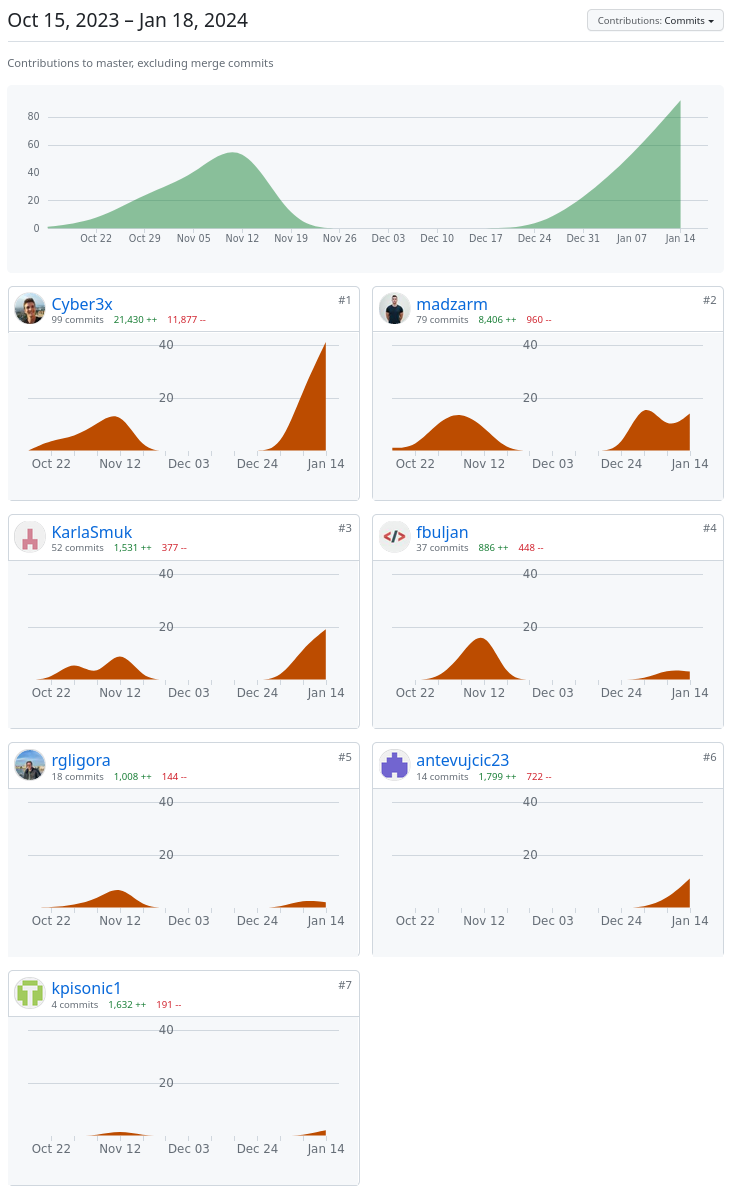
\includegraphics[scale=0.7]{slike/commits.png}
			\centering
			\caption{Grafovi promjena}
			\label{fig:commits}
		\end{figure}
		
		
	



\end{document} %naredbe i tekst nakon ove naredbe ne ulaze u izgrađen dokument 


